\documentclass[12pt]{article}

\usepackage{amsmath,amssymb,amsfonts,mathtools}
\usepackage{physics}
\usepackage{bm}
\usepackage{geometry}
\usepackage{graphicx}
\usepackage{hyperref}
\usepackage{mathrsfs}
\usepackage{tensor}
\usepackage{cite}
\usepackage{setspace}
\usepackage{titlesec}
\usepackage{tikz}
\usepackage{pgfplots}
% pgfplotsset loaded below
\pgfplotsset{compat=1.18}
\usetikzlibrary{arrows.meta,decorations.pathmorphing,decorations.markings,
                calc,shapes.geometric,fit,backgrounds,positioning,
                decorations.pathreplacing,patterns}
\usepackage{xcolor}
\usepackage{booktabs}
\usepackage{array}
\usepackage{caption}
\usepackage{subcaption}
\usepackage{enumitem}
\usepackage{cleveref}
\usepackage{thmtools}
\usepackage{amsthm}
\usepackage{mdframed}

\geometry{margin=1in, top=1.1in, bottom=1.1in}
\setstretch{1.18}

%% Theorem environments
\newtheorem{theorem}{Theorem}[section]
\newtheorem{proposition}[theorem]{Proposition}
\newtheorem{corollary}[theorem]{Corollary}
\newtheorem{lemma}[theorem]{Lemma}
\theoremstyle{definition}
\newtheorem{definition}[theorem]{Definition}
\newtheorem{remark}[theorem]{Remark}

%% Custom colors
\definecolor{rsvpblue}{RGB}{30,80,160}
\definecolor{axiongray}{RGB}{90,90,90}
\definecolor{coherentgreen}{RGB}{20,130,80}
\definecolor{washoutred}{RGB}{180,40,40}

\hypersetup{
  colorlinks=true,
  linkcolor=rsvpblue,
  citecolor=coherentgreen,
  urlcolor=rsvpblue
}

%% Shorthand macros
\newcommand{\kA}{\kappa_A}
\newcommand{\Wrec}{\Delta\eta_{\mathrm{rec}}}
\newcommand{\xirec}{\xi_{\mathrm{rec}}}
\newcommand{\betaobs}{\beta_{\mathrm{obs}}}
\newcommand{\etaLSS}{\eta_{\mathrm{LSS}}}
\newcommand{\etastar}{\eta_\star}
\newcommand{\etaobs}{\eta_0}
\newcommand{\Wpm}{\mathcal{W}_\pm}
\newcommand{\VarW}{\mathrm{Var}_W}
\newcommand{\EW}{\mathbb{E}_W}
\newcommand{\PLSSphi}{\phi_\star}
\newcommand{\gpg}{g_{\phi\gamma}}
\newcommand{\RSVP}{\textsc{rsvp}}
\newcommand{\plenum}{\widetilde{\Gamma}}

%% Section title formatting
\titleformat{\section}{\large\bfseries\color{rsvpblue}}{{\thesection}}{1em}{}
\titleformat{\subsection}{\normalsize\bfseries}{{\thesubsection}}{1em}{}

%%-------------------------------------------------------------------
\title{\textbf{Axial Holonomy and Visibility-Weighted Coherence:\\[4pt]
Cosmic Birefringence in the Relativistic Scalar--Vector Plenum}}

\author{Flyxion}

\date{\today}

\begin{document}
\maketitle
\thispagestyle{empty}

\begin{abstract}
Cosmic birefringence, the rotation of CMB polarization by an angle
$\beta\sim 0.3^\circ$ detected at high significance in recent data
\cite{MinamiKomatsu2020,Eskilt2022,Diego-Palazuelos2023},
is typically attributed to a Chern--Simons coupling between photons
and axion-like particles (ALPs) \cite{Carroll1990,Lue1999}.
Here we reinterpret this phenomenon within the
Relativistic Scalar--Vector Plenum (RSVP)
as a \emph{visibility-weighted axial holonomy} of a
parity-odd sector of the plenum connection.
The polarization rotation angle is the integral of an effective axial
connection $\kappa_A$ along null geodesics;
the washout suppression of polarization amplitude arises from
phase-variance of $\kappa_A$ across the finite recombination visibility
kernel $W(\eta)$ \cite{Fujita2021,Sherfield2023}.
We derive a transport formalism in which mean rotation and depolarization
are governed respectively by the first and second spectral moments of the
axial connection.
The two-field ALP mechanism of Shao--Obata--Zhang \cite{ShaoObataZhang2025}
emerges as a special case of a multi-modal axial sector whose independent
phase components factorize under visibility averaging, yielding the
familiar $\sqrt{N}$ relaxation of washout constraints through variance additivity.
A continuous synchronization model for the parity-odd phase field leads to
a \emph{coherence theorem}: the CMB polarization amplitude imposes a lower
bound on the axial correlation length at $z\approx1100$.
This reframing replaces particle-specific exclusion statements with a
geometric coherence inequality, reveals structural equivalence between
cosmological birefringence and phase-stable photonic computation
\cite{Ozawa2019,Joannopoulos2008}, and predicts discriminants absent
in minimal axion models, including correlations between birefringence
anisotropies and entropy gradients, vorticity statistics, and
multipole-dependent depolarization.
Cosmic birefringence is thus recast as a probe of axial synchronization
in the universe's parity-odd sector rather than solely as evidence for
a propagating pseudoscalar field.
\end{abstract}

\vspace{2pt}
\noindent\rule{\textwidth}{0.4pt}
\tableofcontents
\vspace{4pt}
\noindent\rule{\textwidth}{0.4pt}

\newpage

%%====================================================================
\section{Introduction}
\label{sec:intro}
%%====================================================================

Recent high-significance measurements of cosmic microwave background (CMB)
polarization have revived interest in the possibility of a nonzero global
birefringence angle.
The Planck, WMAP, and ACT data-sets together indicate a rotation
$\beta \approx 0.35^\circ$ at roughly $3\sigma$ significance
\cite{MinamiKomatsu2020,Eskilt2022,Diego-Palazuelos2023,ACTPol2024},
with anisotropic components beginning to be resolved at degree angular scales.
Conventionally, such rotation is modeled through a Chern--Simons coupling
\begin{equation}
  \mathcal{L}_{\mathrm{CS}}
  = -\frac{\gpg}{4}\,\phi\,F_{\mu\nu}\widetilde{F}^{\mu\nu},
  \label{eq:CS_action}
\end{equation}
which leads to a polarization angle proportional to the ALP field
displacement between emission and observation \cite{Carroll1990,Lue1999,
Finelli2009,Pospelov2009}.
Within that framework, the observational bound on polarization amplitude
constrains the oscillation rate and coupling of the pseudoscalar through a
washout condition arising from the finite thickness of recombination
\cite{Fujita2021,Sherfield2023,Murai2023}.

While this particle-based interpretation is algebraically sufficient, it is
not logically necessary.
The observable quantity is a rotation of the photon's transverse polarization
frame, accumulated along null geodesics and weighted by the visibility
function of recombination \cite{Zaldarriaga1998,Hu1997}.
At a structural level this is a \emph{holonomy problem}:
polarization is parallel-transported by an effective optical connection,
and birefringence measures the parity-odd component of that connection
integrated along the path.
The washout bound constrains not a field species per se
but the \emph{phase coherence} of whatever geometric sector sources that
parity-odd projection across the emission kernel.

In this paper we develop that geometric interpretation within the
Relativistic Scalar--Vector Plenum (RSVP) framework.
RSVP posits that cosmological dynamics are governed not solely by a metric
tensor but by a coupled scalar--vector--entropy system $(\Phi,v^\mu,S)$
defined on spacetime \cite{Penrose2004,Verlinde2011,Jacobson1995}.
Gravitational and optical phenomena emerge from the combined geometry of
these fields through effective connections constructed from their gradients
and contractions.
Parity-odd structures arise naturally from pseudoscalar combinations such as
$\varepsilon_{\mu\nu\rho\sigma} k^\mu u^\nu \nabla^\rho S\, v^\sigma$,
where $k^\mu$ is the photon wavevector and $u^\mu$ a comoving four-velocity
\cite{Alexander2009,Nair2010}.

\paragraph{Main results.}
\begin{enumerate}[leftmargin=1.8em,itemsep=2pt]
  \item We derive an \emph{axial transport law} (\cref{sec:geometry})
        expressing CMB polarization rotation as the holonomy of a
        parity-odd sector of the RSVP plenum connection.
  \item We establish a \emph{visibility-weighted holonomy formalism}
        (\cref{sec:visibility}) that identifies the washout bound with a
        spectral coherence constraint on $\kA$.
  \item We show that the two-field ALP mechanism of
        \cite{ShaoObataZhang2025} is a \emph{special case}
        (\cref{sec:multimodal}) of multi-modal axial coherence
        governed by variance additivity.
  \item We prove a \emph{coherence theorem} (\cref{sec:synchronization,
        sec:continuous}) bounding the axial correlation length at
        recombination.
  \item We situate this coherence bound within the broader mathematics
        of \emph{holonomy realizability, conical metric admissibility,
        loop quantum geometry, and supersymmetric gluing}
        (\cref{sec:realizability}), unifying these structures in
        \cref{prop:admissibility}.
  \item We derive an \emph{entropy--coherence inequality}
        (\cref{sec:entropy}) unifying cosmological washout with the
        thermodynamic cost of phase-stable computation.
  \item We identify \emph{observational discriminants}
        (\cref{sec:discriminants}) that distinguish geometric axial
        coherence from free pseudoscalar transport.
\end{enumerate}

\medskip
The paper is organized as follows.
\Cref{sec:geometry} develops the RSVP optical connection and axial
holonomy.
\Cref{sec:visibility} establishes the visibility-weighted formalism and
coherence constraints.
\Cref{sec:multimodal} treats multi-modal factorization and the two-field
mechanism.
\Cref{sec:boundary} discusses foliation structure and local-field dominance.
\Cref{sec:synchronization} introduces the 5D Ising synchronization model.
\Cref{sec:continuous} derives the continuous axial phase model and states
the coherence theorem.
\Cref{sec:realizability} situates the coherence theorem within holonomy
realizability theory, conical metric geometry, loop quantum cosmology,
and supersymmetric gluing.
\Cref{sec:entropy} establishes the entropy--coherence inequality and its
implications for photonic computing.
\Cref{sec:discriminants} presents observational discriminants.
\Cref{sec:conclusion} synthesizes the results.
Technical derivations occupy Appendices \ref{app:transport}--\ref{app:derived}.

%%====================================================================
\section{Geometric Structure of the Relativistic Scalar--Vector Plenum}
\label{sec:geometry}
%%====================================================================

\subsection{Plenum fields and the RSVP connection}

The Relativistic Scalar--Vector Plenum (RSVP) is a geometric field theory
in which spacetime carries three interlocking fields: a scalar density
$\Phi$, a vector flow $v^\mu$, and an entropy density $S$.
The metric $g_{\mu\nu}$ is interpreted as an emergent large-scale descriptor
of averaged plenum structure rather than a primitive background variable
\cite{Jacobson1995,Verlinde2011,Padmanabhan2010}.
Deviations from Levi--Civita transport arise from gradients and vorticity of
$(\Phi,v^\mu,S)$.

The full plenum connection is
\begin{equation}
  \plenum^\mu{}_{\nu\rho}
  = \Gamma^\mu{}_{\nu\rho}
  + \Delta^\mu{}_{\nu\rho}(\Phi,v,S),
  \label{eq:plenum_connection}
\end{equation}
where $\Delta^\mu{}_{\nu\rho}$ represents non-Riemannian structure induced
by plenum ordering \cite{Cartan1922,Hehl1976}.
The correction decomposes irreducibly under spatial inversion into
parity-even and parity-odd sectors.
The parity-odd sector, which we denote $\Delta^{(\mathrm{odd})}$, acts
differently on left- and right-handed polarization states; it is the
geometric locus of cosmic birefringence in RSVP.

\begin{figure}[h]
\centering
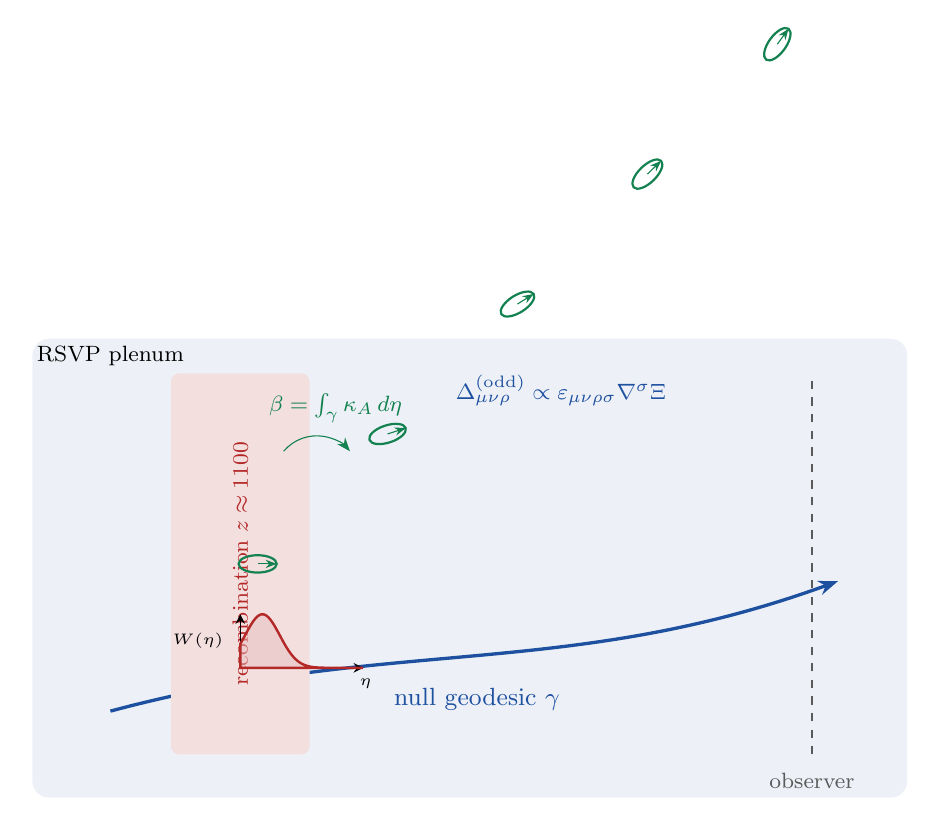
\begin{tikzpicture}[scale=1.1,
  every node/.style={font=\small},
  arrow/.style={-{Stealth[length=6pt]},thick}]

  %% Spacetime background stripe
  \fill[rsvpblue!8, rounded corners=6pt]
    (-0.6,-0.5) rectangle (9.5,4.8);

  %% Null geodesic
  \draw[rsvpblue, very thick, -{Stealth[length=7pt]}]
    (0.3,0.5) to[out=15,in=200] node[midway,below=8pt,rsvpblue]
    {null geodesic $\gamma$} (8.7,2.0);

  %% LSS band
  \fill[washoutred!15, rounded corners=3pt]
    (1.0,0.0) rectangle (2.6,4.4);
  \node[washoutred, rotate=90, font=\footnotesize] at (1.8,2.2)
    {recombination $z\approx1100$};

  %% Observer vertical line
  \draw[axiongray, dashed, thick] (8.4,0.0) -- (8.4,4.4);
  \node[axiongray, font=\footnotesize] at (8.4,-0.3) {observer};

  %% Polarization ellipses along ray
  \foreach \x/\ang in {2.0/0, 3.5/18, 5.0/32, 6.5/44, 8.0/54}{
    \begin{scope}[shift={(\x, 0.5+(\x-0.3)*0.178)}, rotate=\ang]
      \draw[coherentgreen, thick] (0,0) ellipse (0.22 and 0.10);
      \draw[coherentgreen,-{Stealth[length=4pt]},thin]
        (0,0) -- (0.22,0);
    \end{scope}
  }

  %% Rotation annotation
  \draw[coherentgreen, -{Stealth[length=5pt]}]
    (2.3,3.5) arc(140:40:0.5);
  \node[coherentgreen, font=\footnotesize] at (2.9,4.0)
    {$\beta = \int_\gamma \kA\,d\eta$};

  %% Visibility kernel inset
  \begin{axis}[
    at={(1.8cm,1.0cm)}, anchor=south west,
    width=3.0cm, height=2.2cm,
    axis x line=bottom, axis y line=left,
    xtick=\empty, ytick=\empty,
    xlabel={\tiny $\eta$},
    ylabel={\tiny $W(\eta)$},
    xlabel style={font=\tiny, at={(axis description cs:1.02,0.0)}},
    ylabel style={font=\tiny, rotate=-90},
    domain=0:1, samples=80,
    clip=false
  ]
    \addplot[washoutred, thick, fill=washoutred!30, fill opacity=0.5]
      {exp(-25*(x-0.18)^2)} \closedcycle;
  \end{axis}

  %% Labels
  \node[font=\footnotesize] at (0.3,4.6) {RSVP plenum};
  \node[font=\footnotesize,rsvpblue] at (5.5,4.2)
    {$\Delta^{(\mathrm{odd})}_{\mu\nu\rho}\propto
      \varepsilon_{\mu\nu\rho\sigma}\nabla^\sigma\Xi$};
\end{tikzpicture}
\caption{Schematic of axial holonomy along a null geodesic $\gamma$
  in the RSVP plenum.
  Photon polarization (green ellipses) rotates by an angle
  $\beta=\int_\gamma\kA\,d\eta$ controlled by the parity-odd projection
  $\kA$ of the plenum connection $\Delta^{(\mathrm{odd})}$.
  The red band marks the recombination visibility kernel $W(\eta)$;
  phase oscillations faster than $\Wrec$ contribute to depolarization
  rather than coherent rotation.}
\label{fig:holonomy_schematic}
\end{figure}

\subsection{Polarization transport equation}

Let $k^\mu$ be the null tangent to $\gamma$ and $P^\mu$ a transverse
polarization vector with $P^\mu k_\mu=0$.
Standard geometric optics gives $k^\nu\nabla_\nu P^\mu=0$
\cite{MisnerThorneWheeler,Grasso2018,Oancea2020};
in RSVP the transport is instead
\begin{equation}
  k^\nu\widetilde{\nabla}_\nu P^\mu = 0,
\end{equation}
where $\widetilde{\nabla}$ uses the full plenum connection
\eqref{eq:plenum_connection}.
Projecting onto the two-dimensional screen bundle
$\{e_1^\mu,e_2^\mu\}$ orthogonal to $k^\mu$ and $u^\mu$, the parity-odd
sector induces an effective scalar angular velocity
\begin{equation}
  \frac{d\theta}{d\lambda} = \kA(\lambda),
  \qquad
  \kA(\lambda)
  = \Pi^\mu{}_a\,\Pi^\nu{}_b\,\epsilon^{ab}\,k^\rho
    \Delta_{\mu\nu\rho}^{(\mathrm{odd})},
  \label{eq:kA_def}
\end{equation}
so that the accumulated axial holonomy along $\gamma$ is
\begin{equation}
  \boxed{
  H_A[\gamma]
  = \int_{\etaLSS}^{\etaobs}
    \kA(\eta,x(\eta))\,d\eta.}
  \label{eq:holonomy}
\end{equation}
This is structurally identical to the Chern--Simons result
$\beta=\frac{1}{2}\gpg(\phi_{\etaobs}-\phi_{\etaLSS})$
under the identification
\begin{equation}
  \kA \;\longleftrightarrow\; \tfrac{1}{2}\gpg\,\partial_\eta\phi,
  \label{eq:identification}
\end{equation}
but now $\kA$ is a projection of plenum geometry rather than a derivative
of a particle field.

\subsection{Internal origin of the parity-odd sector}

A minimal covariant parity-odd connection compatible with RSVP fields is
\begin{equation}
  \Delta^{(\mathrm{odd})}_{\mu\nu\rho}
  = \alpha\,\varepsilon_{\mu\nu\rho\sigma}\,\nabla^\sigma\Xi(\Phi,v,S),
  \label{eq:Delta_odd}
\end{equation}
where $\alpha$ is a coupling scale and $\Xi$ is any pseudoscalar functional
of the plenum.
The canonical choice coupling entropy gradients to vorticity is
\begin{equation}
  \Xi = \nabla_\mu S\,\omega^\mu,
  \qquad
  \omega^\mu = \varepsilon^{\mu\nu\rho\sigma}u_\nu\nabla_\rho v_\sigma,
  \label{eq:Xi}
\end{equation}
which is manifestly parity-odd and depends only on plenum kinematics,
not on any new fundamental field
\cite{Alexander2009,Nair2010,Maleknejad2013}.
The axion model is recovered when $\Xi\to\phi$ is promoted to an independent
dynamical pseudoscalar with the action \eqref{eq:CS_action}.
RSVP treats $\Xi$ as emergent from plenum ordering.

%%====================================================================
\section{Visibility-Weighted Holonomy and Coherence Constraints}
\label{sec:visibility}
%%====================================================================

\subsection{Observable polarization}

CMB polarization is generated across a finite conformal time interval
centered at recombination \cite{Zaldarriaga1998,Hu1997,Kosowsky1996}.
Let $W(\eta)$ be the visibility function, normalized to unity, with
characteristic width $\Wrec\approx10\,\mathrm{Mpc}/h$ at
$z\approx1100$ \cite{Weinberg2008}.
Defining complex polarization $P_\pm=Q\pm iU$, the observed polarization is
\begin{equation}
  P_\pm^{\mathrm{obs}}(\hat{n})
  = \int d\eta\,W(\eta)\,
    e^{\pm 2i\beta(\eta,\hat{n})}\,P_\pm^{(0)}(\eta,\hat{n}),
  \label{eq:Pobs}
\end{equation}
where $\beta(\eta,\hat{n})=\int_\eta^{\etaobs}\kA(\eta',x(\eta'))d\eta'$
is the holonomy from emission time $\eta$ to the observer.
Factoring out the slowly varying intrinsic polarization,
\begin{equation}
  P_\pm^{\mathrm{obs}} = \Wpm(\hat{n})\,P_\pm^{(0)}(\etastar,\hat{n}),
  \quad
  \Wpm(\hat{n}) = \int d\eta\,W(\eta)\,e^{\pm2i\beta(\eta,\hat{n})}.
  \label{eq:Wpm}
\end{equation}
The washout effect is $|\Wpm|<1$ due to phase decoherence across
the kernel \cite{Fujita2021,Sherfield2023,Murai2023}.

\subsection{Spectral decomposition and Bessel suppression}

Decompose $\kA$ into a coherent component and oscillatory modes:
\begin{equation}
  \kA(\eta) = \kappa_0(\eta)
    + \sum_k a_k\cos(\omega_k\eta+\varphi_k).
  \label{eq:kA_decomp}
\end{equation}
The holonomy becomes
\begin{equation}
  \beta(\eta) = \bar\beta
    + \sum_k A_k\sin(\omega_k\eta+\varphi_k),
  \qquad
  A_k=\frac{a_k}{\omega_k},
  \label{eq:beta_decomp}
\end{equation}
where $\bar\beta=\int_{\etastar}^{\etaobs}\kappa_0d\eta'$.
For modes with $\omega_k\Wrec\gg1$ the integral over $W(\eta)$
reduces to a Bessel-$J_0$ suppression
\cite{Abramowitz1972,Watson1944}:
\begin{equation}
  \int d\eta\,W(\eta)\,e^{iA_k\sin(\omega_k\eta)}
  \approx J_0(A_k).
\end{equation}
With spectrally separated modes, the full suppression factorizes:
\begin{equation}
  \Wpm \approx e^{\pm2i\bar\beta}\prod_k J_0(2A_k).
  \label{eq:Wpm_bessel}
\end{equation}
Expanding for small $A_k$:
\begin{equation}
  |\Wpm| \approx 1 - 2\sum_k A_k^2 + \mathcal{O}(A_k^4),
  \label{eq:Wpm_expand}
\end{equation}
yielding the fundamental \emph{coherence inequality}
\begin{equation}
  \boxed{
  \sum_k A_k^2 \lesssim \epsilon_{\mathrm{wash}},}
  \label{eq:coherence_ineq}
\end{equation}
where $\epsilon_{\mathrm{wash}}$ is the observationally determined upper bound
on depolarization \cite{MinamiKomatsu2020,Eskilt2022,Sherfield2023}.
This bounds the spectral variance of $\kA$ at
frequencies exceeding $\Wrec^{-1}$, not the mean coherent component
$\bar\beta$.

\begin{figure}[h]
\centering
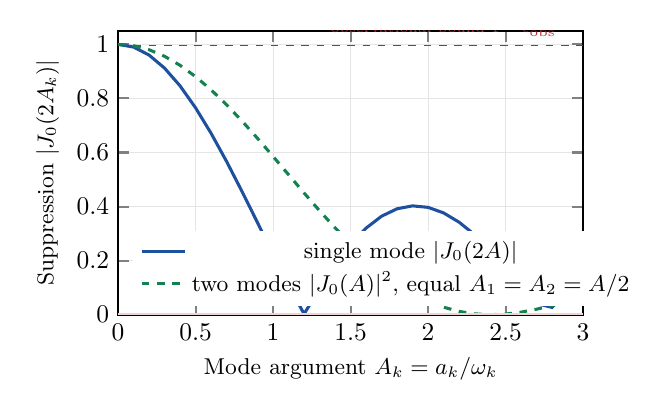
\begin{tikzpicture}[scale=0.92]
  \begin{axis}[
    width=8cm, height=5.5cm,
    xlabel={Mode argument $A_k = a_k/\omega_k$},
    ylabel={Suppression $|J_0(2A_k)|$},
    xmin=0, xmax=3.0,
    ymin=0, ymax=1.05,
    xtick={0,0.5,1.0,1.5,2.0,2.5,3.0},
    ytick={0,0.2,0.4,0.6,0.8,1.0},
    grid=both,
    grid style={draw=gray!20},
    legend pos=south west,
    legend style={font=\small, draw=none, fill=white},
    axis line style={thick},
    tick style={thick},
    label style={font=\small},
  ]
    %% Single-field J0 (precomputed from scipy)
    \addplot[rsvpblue, very thick]
      coordinates {
        (0.0,1.0)(0.1,0.99)(0.2,0.9604)(0.3,0.912)(0.4,0.8463)
        (0.5,0.7652)(0.6,0.6711)(0.7,0.5669)(0.8,0.4554)(0.9,0.34)
        (1.0,0.2239)(1.1,0.1104)(1.2,0.0025)(1.3,0.0968)(1.4,0.185)
        (1.5,0.2601)(1.6,0.3202)(1.7,0.3643)(1.8,0.3918)(1.9,0.4026)
        (2.0,0.3971)(2.1,0.3766)(2.2,0.3423)(2.3,0.2961)(2.4,0.2404)
        (2.5,0.1776)(2.6,0.1103)(2.7,0.0412)(2.8,0.027)(2.9,0.0917)
        (3.0,0.1506)};
    \addlegendentry{single mode $|J_0(2A)|$}

    %% Two-field product (equal amplitudes, precomputed)
    \addplot[coherentgreen, very thick, dashed]
      coordinates {
        (0.0,1.0)(0.1,0.995)(0.2,0.9801)(0.3,0.9558)(0.4,0.9224)
        (0.5,0.8807)(0.6,0.8318)(0.7,0.7765)(0.8,0.7162)(0.9,0.6521)
        (1.0,0.5855)(1.1,0.5179)(1.2,0.4504)(1.3,0.3845)(1.4,0.3213)
        (1.5,0.262)(1.6,0.2074)(1.7,0.1584)(1.8,0.1156)(1.9,0.0794)
        (2.0,0.0501)(2.1,0.0278)(2.2,0.0122)(2.3,0.0031)(2.4,0.0)
        (2.5,0.0023)(2.6,0.0094)(2.7,0.0203)(2.8,0.0342)(2.9,0.0503)
        (3.0,0.0676)};
    \addlegendentry{two modes $|J_0(A)|^2$, equal $A_1=A_2=A/2$}

    %% Observational bound region
    \addplot[fill=washoutred!20, draw=none, domain=0:3, samples=2]
      {0.0058} \closedcycle;
    \draw[washoutred, dashed] (axis cs:0,0.9942) -- (axis cs:3,0.9942)
      node[pos=0.7, above, font=\tiny, washoutred]
      {observational bound $1-\epsilon_\mathrm{obs}$};
  \end{axis}
\end{tikzpicture}
\caption{Washout suppression factor as a function of mode amplitude $A_k$.
  Blue: single-mode Bessel factor $|J_0(2A)|$.
  Green dashed: two-mode product $|J_0(A)|^2$ for equal-amplitude modes
  each contributing $A_k=A/2$.
  The two-mode configuration achieves the same mean rotation at reduced
  depolarization.
  The red dashed line marks the observational amplitude bound
  $|\mathcal{W}_\pm|\geq0.9942$ from \protect\cite{Sherfield2023}.}
\label{fig:bessel_washout}
\end{figure}

%%====================================================================
\section{Multi-Modal Axial Connection and Factorized Dephasing}
\label{sec:multimodal}
%%====================================================================

\subsection{Two-field mechanism as special case}

In the Shao--Obata--Zhang scenario \cite{ShaoObataZhang2025}, two ALP
fields $\phi_1,\phi_2$ with common photon coupling contribute
\begin{equation}
  \kA(\eta) = -\tfrac{1}{2}\gpg
    \sum_{i=1}^2\Phi_i m_i\sin(m_i\eta+\alpha_i),
  \label{eq:kA_twofield}
\end{equation}
with mode amplitudes $A_i=\tfrac{1}{2}\gpg\Phi_i$ and
frequencies $\omega_i=m_i$.
When $|m_1-m_2|\gg\Wrec^{-1}$, cross-terms average out and
\begin{equation}
  \Wpm \approx e^{\pm2i\bar\beta}\,J_0(2A_1)\,J_0(2A_2).
  \label{eq:Wpm_twofield}
\end{equation}
This is the RSVP multi-modal result \eqref{eq:Wpm_bessel} for $k=1,2$:
the two-field mechanism is a special instance of a two-mode axial sector.

\subsection{Variance additivity and the $\sqrt{N}$ relief}

For small amplitudes, the distinction between single- and two-mode washout
is algebraic:
\begin{align}
  \text{single mode:}&
    \quad J_0(2A)\approx1-2A^2,
    \quad A=A_1+A_2,
    \label{eq:single_small}\\
  \text{two modes:}&
    \quad J_0(2A_1)J_0(2A_2)\approx1-2(A_1^2+A_2^2).
    \label{eq:two_small}
\end{align}
The single-mode suppression at fixed total amplitude scales as
$(A_1+A_2)^2$; the two-mode product scales as $A_1^2+A_2^2$.
The difference $2A_1A_2$ is the cross-term that vanishes when the modes
oscillate incoherently across the visibility kernel.
For equal amplitudes $A_1=A_2\equiv\bar{A}$,
\begin{equation}
  \frac{\text{two-mode washout}}{\text{single-mode washout}}
  = \frac{2\bar{A}^2}{4\bar{A}^2} = \tfrac{1}{2},
\end{equation}
giving a $\sqrt{2}$ improvement in coherent rotation per unit depolarization
budget.
For $N$ equal-amplitude modes:
\begin{equation}
  \frac{\langle\beta\rangle}{\sqrt{\VarW[\Theta]}}
  \propto \sqrt{N}.
  \label{eq:sqrtN}
\end{equation}
This is not a special property of axions but a \emph{universal consequence
of variance additivity under independent phase modes} \cite{Rice1954,Papoulis1991}.

\begin{figure}[h]
\centering
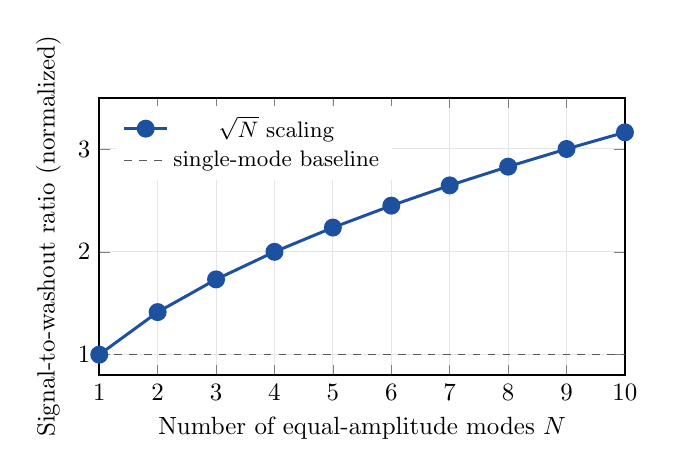
\begin{tikzpicture}[scale=0.90]
  \begin{axis}[
    width=9cm, height=5.5cm,
    xlabel={Number of equal-amplitude modes $N$},
    ylabel={Signal-to-washout ratio (normalized)},
    xmin=1, xmax=10,
    ymin=0.8, ymax=3.5,
    xtick={1,2,3,4,5,6,7,8,9,10},
    grid=both,
    grid style={draw=gray!20},
    legend pos=north west,
    legend style={font=\small, draw=none},
    axis line style={thick},
  ]
    \addplot[rsvpblue, very thick, mark=*, mark size=3pt,
             mark options={fill=rsvpblue}]
      coordinates {
        (1,1.0)(2,1.414)(3,1.732)(4,2.0)(5,2.236)
        (6,2.449)(7,2.646)(8,2.828)(9,3.0)(10,3.162)
      };
    \addlegendentry{$\sqrt{N}$ scaling}
    \addplot[axiongray, dashed, domain=1:10, samples=10]
      {1.0};
    \addlegendentry{single-mode baseline}
  \end{axis}
\end{tikzpicture}
\caption{Signal-to-washout ratio $\langle\beta\rangle/\sqrt{\VarW[\Theta]}$
  normalized to unity for $N=1$, showing universal $\sqrt{N}$ scaling
  from variance additivity under $N$ independent axial modes.
  The two-field mechanism of \protect\cite{ShaoObataZhang2025}
  corresponds to $N=2$.}
\label{fig:sqrtN}
\end{figure}

%%====================================================================
\section{Boundary Dominance and Foliation Structure}
\label{sec:boundary}
%%====================================================================

\subsection{Origin of the boundary-term structure}

The standard axion result $\beta=\tfrac{1}{2}\gpg(\phi_{\etaobs}-\phi_{\etaLSS})$
is a boundary term.
Within RSVP this structure is not an artifact of the axion equation of motion
but a \emph{structural consequence of visibility-weighted holonomy}.

Interchanging integration order in $\betaobs=\int W(\eta)\beta(\eta)d\eta$:
\begin{equation}
  \betaobs
  = \int\kA(\eta')\,\mathcal{F}(\eta')\,d\eta',
  \qquad
  \mathcal{F}(\eta') = \int_{\etaLSS}^{\eta'} W(\eta)\,d\eta.
  \label{eq:boundary_deriv}
\end{equation}
The cumulative visibility $\mathcal{F}(\eta')$ rises sharply from
$0$ to $1$ across $\Wrec$ and remains unity thereafter.
For oscillatory modes with $\omega_k\Wrec\gg1$, the emission-window
contribution $\int_{\etaLSS}^{\etastar}\kA\,\mathcal{F}\,d\eta'$ averages to
zero, leaving
\begin{equation}
  \betaobs \approx \int_{\etastar}^{\etaobs}\kA(\eta')\,d\eta',
  \label{eq:boundary_result}
\end{equation}
a \emph{post-recombination} integral depending on the observer-side
plenum state \cite{Fujita2021,Murai2023}.

\subsection{Local-field dominance as a structural fact}

When modes oscillate many times between $\etastar$ and $\etaobs$,
the LSS contribution $\int^{\etastar}\kA\,d\eta'$ is effectively a random
phase in the ensemble:
\begin{equation}
  \left\langle\int_{\etaLSS}^{\etastar}
    \kA(\eta')\,\mathcal{F}(\eta')\,d\eta'\right\rangle = 0.
\end{equation}
The observed isotropic $\beta$ measures the axial state of the plenum
at the \emph{observer's foliation}---a single evaluation point---not
an integrated history.
This makes local-field dominance not mysterious but structural:
it is what any ordering-based observable does when the source kernel
is broad relative to the medium's oscillation period
\cite{Zaldarriaga1998,Sherfield2023}.

%%====================================================================
\section{A Five-Dimensional Ising Synchronization Model}
\label{sec:synchronization}
%%====================================================================

The coherence constraint \eqref{eq:coherence_ineq} motivates a
constructive question: what class of mesoscopic dynamics can generate
a parity-odd sector with tunable correlation length?
We introduce a five-dimensional Ising-type synchronization model
to answer this.

\subsection{Lattice construction}

Let $\Lambda\subset\mathbb{Z}^5$ be a hypercubic lattice with sites
$x=(n_0,n_1,n_2,n_3,n_4)$, where the first four coordinates represent
a coarse-grained comoving spacetime lattice and $n_4$ indexes an
internal axial layer.
At each site we place an Ising spin
$\sigma_x\in\{-1,+1\}$ representing the sign of the local
parity-odd plenum response \cite{Ising1925,Onsager1944}.

The anisotropic Hamiltonian is
\begin{equation}
  \mathcal{H}[\sigma]
  = -\sum_{x\in\Lambda}
    \left(
      \sum_{\mu=0}^{3} J_\mu\,\sigma_x\sigma_{x+\hat\mu}
      + J_4\,\sigma_x\sigma_{x+\hat4}
    \right)
  -\sum_{x\in\Lambda} h_x\sigma_x,
  \label{eq:Ising_H}
\end{equation}
where $J_4$ controls axial-layer synchronization and
$h_x\propto\Xi(x)$ encodes slow RSVP biases from the plenum
pseudoscalar \eqref{eq:Xi}.

The coarse-grained axial integrand along a null ray is
\begin{equation}
  \kA(\eta) = \kappa_0\,m(\eta),
  \qquad
  m(\eta) = \mathbb{E}[\sigma_{x(\eta)}],
\end{equation}
with correlation function
\begin{equation}
  C(\Delta\eta) = \mathbb{E}[m(\eta)m(\eta+\Delta\eta)]
                - \mathbb{E}[m]^2.
\end{equation}

\subsection{Washout as a correlation-length constraint}

For exponential decay $C(\Delta\eta)\sim e^{-|\Delta\eta|/\xirec}$,
the visibility-weighted variance scales as
\begin{equation}
  \VarW[\Theta]
  \sim 4\kappa_0^2
       \int d\eta\,d\eta'\,W(\eta)W(\eta')\,
       e^{-|\eta-\eta'|/\xirec}.
  \label{eq:Var_xi}
\end{equation}
The qualitative regime distinction is immediate (see \cref{fig:regimes}):
\begin{itemize}[nosep]
  \item $\xirec\gg\Wrec$: coherent sector; exponential $\approx1$ over
        $\mathrm{supp}(W)$; small variance, large mean rotation.
  \item $\xirec\ll\Wrec$: incoherent sector; variance extensive in
        sub-intervals; strong depolarization, suppressed mean.
\end{itemize}

\begin{figure}[h]
\centering
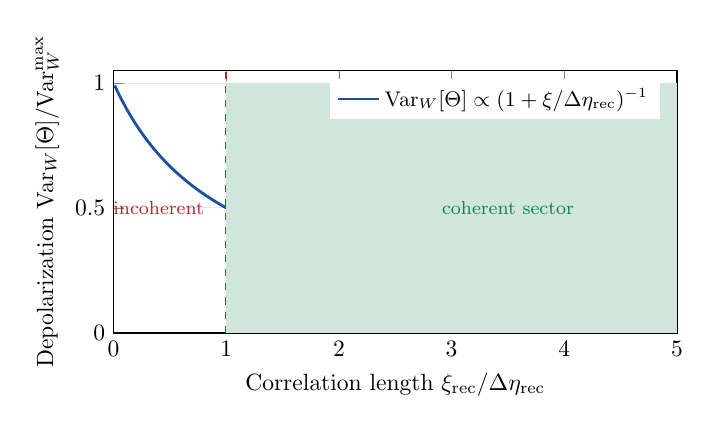
\begin{tikzpicture}[scale=0.85]
  \begin{axis}[
    width=10cm, height=5.5cm,
    xlabel={Correlation length $\xi_{\mathrm{rec}}/\Delta\eta_{\mathrm{rec}}$},
    ylabel={Depolarization $\VarW[\Theta]/\VarW^{\max}$},
    xmin=0, xmax=5,
    ymin=0, ymax=1.05,
    xtick={0,1,2,3,4,5},
    xticklabels={$0$,$1$,$2$,$3$,$4$,$5$},
    grid=both,
    grid style={draw=gray!20},
    legend pos=north east,
    legend style={font=\small, draw=none},
    axis line style={thick},
  ]
    %% Approximation: Var ~ 1/(1 + xi)
    \addplot[rsvpblue, very thick, domain=0.01:5, samples=200]
      {1/(1+x)};
    \addlegendentry{$\VarW[\Theta]\propto(1+\xi/\Wrec)^{-1}$}

    %% Threshold
    \draw[washoutred, dashed, thick]
      (axis cs:1,0) -- (axis cs:1,1.05);
    \node[washoutred, font=\small, rotate=90]
      at (axis cs:1.12,0.55) {coherence threshold};

    %% Shading
    \addplot[fill=coherentgreen!20, draw=none, domain=1:5, samples=2]
      {1.0} \closedcycle;
    \node[coherentgreen, font=\footnotesize] at (axis cs:3.5,0.5)
      {coherent sector};
    \node[washoutred, font=\footnotesize] at (axis cs:0.4,0.5)
      {incoherent};
  \end{axis}
\end{tikzpicture}
\caption{Depolarization $\VarW[\Theta]$ as a function of the ratio
  $\xirec/\Wrec$.
  The washout bound requires $\xirec\gtrsim\Wrec$ (green region).
  The boundary at $\xirec=\Wrec$ marks the transition from coherent
  rotation to dominant depolarization.}
\label{fig:regimes}
\end{figure}

The washout observational bound therefore constrains not a particle
mass but the axial synchronization length of the plenum at
$z\approx1100$ \cite{KosterlitzThouless1973,Goldenfeld1992}.

%%====================================================================
\section{Continuous Axial Phase Synchronization and the Coherence Theorem}
\label{sec:continuous}
%%====================================================================

\subsection{XY synchronization model}

The discrete Ising model captures combinatorial synchronization but
suppresses the essential $S^1$ geometry of polarization.
We replace it with an anisotropic XY model \cite{KosterlitzThouless1973}
with a continuous phase field $\theta(x)\in S^1$.
In the continuum limit the free energy functional is
\begin{equation}
  \mathcal{F}[\theta]
  = \int d^4x\,dn_4
    \left[
      \frac{K}{2}(\partial_\mu\theta)^2
      + \frac{K_4}{2}(\partial_{n_4}\theta)^2
      - \lambda\,\Xi(x)\cos\theta
    \right],
  \label{eq:XY_free_energy}
\end{equation}
with $\Xi$ the plenum pseudoscalar \eqref{eq:Xi}.
The axial projection is $\kA=\kappa_0\partial_\eta\theta$,
recovering the boundary structure
$\beta(\eta)=\kappa_0[\theta(\etaobs)-\theta(\eta)]$.

\subsection{Correlation function and variance}

Decomposing $\theta=\bar\theta+\delta\theta$ with $\langle\delta\theta\rangle=0$,
the suppression factor is
\begin{equation}
  |\Wpm| = \exp\!\left(-2\kappa_0^2\VarW[\delta\theta]\right),
  \label{eq:Wpm_gauss}
\end{equation}
with
\begin{equation}
  \VarW[\delta\theta]
  = \int d\eta\,d\eta'\,W(\eta)W(\eta')
    \langle\delta\theta(\eta)\delta\theta(\eta')\rangle.
  \label{eq:Var_gaussian}
\end{equation}
For an exponential two-point function
$\langle\delta\theta(\eta)\delta\theta(\eta')\rangle
  \propto e^{-|\eta-\eta'|/\xirec}$:
\begin{align}
  \VarW[\delta\theta]
  &\sim \frac{\Wrec}{\xirec}
  \quad(\xirec\ll\Wrec),
  \label{eq:Var_incoherent}\\
  \VarW[\delta\theta]
  &\sim \mathrm{const}
  \quad(\xirec\gg\Wrec).
  \label{eq:Var_coherent}
\end{align}

\subsection{The Coherence Theorem}

\begin{theorem}[Coherence Bound on the Parity-Odd Plenum Sector]
\label{thm:coherence}
Let $\kA(\eta)=\kappa_0\partial_\eta\theta(\eta)$ be the axial projection
of the RSVP connection along null geodesics, where $\theta$ has
correlation length $\xirec$ across the recombination visibility kernel
of width $\Wrec$.

\begin{enumerate}[label=\textup{(\roman*)}]
  \item \emph{Coherent regime.}
        If $\xirec\gg\Wrec$, then
        $\betaobs\approx\kappa_0(\theta(\etaobs)-\theta(\etastar))$
        with negligible washout.
  \item \emph{Incoherent regime.}
        If $\xirec\ll\Wrec$, then polarization amplitude is suppressed by
        $|\Wpm|=\exp(-2\kappa_0^2\VarW[\delta\theta])$
        with $\VarW[\delta\theta]\propto\Wrec/\xirec$.
  \item \emph{Observational bound.}
        The empirical constraint $|\Wpm|\geq1-\epsilon_{\mathrm{obs}}$
        \cite{MinamiKomatsu2020,Sherfield2023} implies
        \begin{equation}
          \boxed{\xirec \gtrsim
                \frac{2\kappa_0^2\Wrec}{\epsilon_{\mathrm{obs}}}.}
          \label{eq:coherence_bound}
        \end{equation}
\end{enumerate}
\end{theorem}

\begin{proof}
Parts (i) and (ii) follow from inserting the exponential correlation
model into \eqref{eq:Var_gaussian} and evaluating the asymptotic limits.
Part (iii) follows by combining \eqref{eq:Wpm_gauss} with
$|\Wpm|\geq1-\epsilon_{\mathrm{obs}}$, which gives
$\VarW[\delta\theta]\leq\epsilon_{\mathrm{obs}}/(2\kappa_0^2)$,
and substituting the scaling \eqref{eq:Var_incoherent}.
\end{proof}

\begin{remark}
  Inequality \eqref{eq:coherence_bound} is a \emph{geometric observational
  bound on the coherence of the parity-odd plenum sector at recombination}.
  It does not specify the microphysical origin of $\theta$ but constrains
  its correlation structure, replacing particle-exclusion statements with
  a synchronization-length bound.
\end{remark}

%%====================================================================
\section{Entropy--Coherence Inequality and Implications for Computing}
\label{sec:entropy}
%%====================================================================

\subsection{Phase-coherent transport as holonomy}

The coherence theorem identifies a universal structure: controlled
holonomy across a finite integration kernel requires
$\VarW[\delta\Theta]\lesssim\varepsilon$.
This structure appears in any system in which computation is performed
through controlled phase transport, with the cosmological and engineering
identifications
\begin{equation}
  \eta\leftrightarrow t,
  \quad
  W(\eta)\leftrightarrow K(t),
  \quad
  \kA(\eta)\leftrightarrow\Omega(t),
  \label{eq:cosmo_compute_map}
\end{equation}
where $K(t)$ is the detector/device integration kernel and $\Omega(t)$
the phase rotation rate \cite{Ozawa2019,Joannopoulos2008,Shen2010}.

\subsection{The entropy--coherence inequality}

For a synchronization field with diffusion coefficient
$D_\theta=k_BT/\gamma$ (Einstein relation \cite{Kubo1966}),
the phase variance over a kernel of width $\Delta t$ scales as
$\VarW[\delta\Theta]\sim2D_\theta\Delta t$.
The coherence condition becomes
\begin{equation}
  \frac{k_BT}{\gamma}\Delta t \lesssim \varepsilon,
  \label{eq:entropy_coherence}
\end{equation}
or equivalently
\begin{equation}
  \boxed{
  \gamma \geq \frac{k_BT\Delta t}{\varepsilon}.}
  \label{eq:damping_bound}
\end{equation}
The entropy export rate (through damping $\gamma$) must exceed a threshold
proportional to temperature and integration time in order to maintain
coherent phase rotation \cite{Seifert2012,Parrondo2015}.

\subsection{Multi-modal architectures}

For $N$ modes with independent diffusion coefficients $D_a$,
$\VarW=\sum_aD_a\Delta t$ while the coherent mean scales as
$\sum_a\bar\Theta_a$.
The multi-modal entropy--coherence inequality is
\begin{equation}
  \sum_{a=1}^N \frac{k_BT_a}{\gamma_a}\Delta t \lesssim \varepsilon,
  \label{eq:multimodal_entropy}
\end{equation}
which may be satisfied with weaker individual damping when modes are
independent.
This is the thermodynamic statement of the $\sqrt{N}$ signal-to-noise
improvement \eqref{eq:sqrtN}: distributing the phase holonomy across $N$
weakly coupled channels requires proportionally less entropy export per
channel \cite{Proesmans2020}.

\begin{table}[h]
\centering
\small
\renewcommand{\arraystretch}{1.35}
\begin{tabular}{>{\bfseries}lcc}
  \toprule
  & Cosmological & Photonic/thermodynamic \\
  \midrule
  Phase variable & $\theta(\eta)$ (axial plenum) & $\theta(t)$ (optical mode) \\
  Rotation rate & $\kA$ & $\Omega(t)$ \\
  Integration kernel & $W(\eta)$ (visibility) & $K(t)$ (detector window) \\
  Kernel width & $\Wrec$ & $\Delta t$ \\
  Coherence bound & $\xirec\gg\Wrec$ & $\xi_c\gg\Delta t$ \\
  Entropy constraint & $\gamma\geq k_BT\Wrec/\varepsilon$ & $\gamma\geq k_BT\Delta t/\varepsilon$ \\
  \bottomrule
\end{tabular}
\caption{Structural correspondence between the cosmological washout constraint
  and the engineering coherence limit for phase-based computation.
  Both are governed by the same entropy--coherence inequality
  \eqref{eq:damping_bound}.}
\label{tab:analogy}
\end{table}

%%====================================================================
\section{Holonomy Realizability, Conical Metrics, and Quantum Geometry}
\label{sec:realizability}
%%====================================================================

\subsection{Branch data and holonomy realizability}

The reinterpretation of cosmic birefringence as a visibility-weighted axial holonomy places the problem squarely within a classical mathematical tradition concerned with the realizability of prescribed holonomy data. In the theory of branched coverings of the Riemann sphere, the branch data of a rational map encodes the local monodromy around each branch point, and the realizability problem asks whether a specified collection of partitions can arise from a global holomorphic map. Song and Xu establish that for rational functions with more than three branch points, realizability is governed not merely by combinatorial compatibility but by a sharp inequality involving the maximal branching order and a greatest-common-divisor constraint \cite{SongXu2019}. The obstruction is therefore global and arithmetic: the monodromy must assemble coherently into a globally defined map.

The axial sector of the Relativistic Scalar--Vector Plenum admits an analogous interpretation. The parity-odd projection of the plenum connection defines a $U(1)$-valued holonomy along null geodesics. The recombination visibility kernel enforces a finite integration interval, and the observable birefringence is the weighted monodromy accumulated across that interval. The washout bound is thus not a constraint on a field amplitude but on the realizability of a global holonomy under finite-thickness averaging: just as branch partitions must satisfy global arithmetic constraints to define a rational map, the spectral components of $\kA$ must satisfy the coherence inequality \eqref{eq:coherence_ineq} to define a non-depolarizing holonomy.

More precisely, let $\rho: \pi_1(M\setminus\Sigma)\to U(1)_A$ be the holonomy representation of the axial connection, where $\Sigma$ denotes the recombination hypersurface viewed as a codimension-one locus. The washout observable $|\Wpm|$ measures the modulus of the $W$-averaged holonomy character $\chi(\rho)$. For $|\Wpm|\to0$, the representation $\rho$ becomes effectively non-abelian over the visibility kernel: phase variance dominates and the holonomy is not realizable as a coherent rotation. The observational bound $|\Wpm|\geq1-\epsilon_{\mathrm{obs}}$ is therefore an \emph{abelian realizability condition} on $\rho$ under the kernel measure, directly analogous to the branching-order bound of \cite{SongXu2019}.

\subsection{Conical holonomy and the Mondello--Panov admissibility condition}

The parallel deepens in the spherical metric problem. For a 2-sphere endowed with conical singularities of prescribed angles $\theta_i$, existence of a spherical metric of curvature $+1$ requires not only the Gauss--Bonnet positivity condition $\sum_i(2\pi-\theta_i)<4\pi$ but also additional holonomy inequalities expressed in terms of $\ell^1$ distances from integer lattices \cite{MondelloPanov2016,Eremenko2004,Dey2018}. When equality holds in these inequalities, the monodromy representation is coaxial, meaning all generators fix a common axis in $SU(2)$.

In the birefringence context, the polarization holonomy acts on the two-dimensional screen space as an element of $SO(2)\cong U(1)$. A purely isotropic rotation---uniform $\beta(\hat{n})=\bar\beta$ over the sky---corresponds precisely to a coaxial holonomy in polarization space. The empirical near-isotropy of the observed birefringence angle \cite{MinamiKomatsu2020,Eskilt2022,Diego-Palazuelos2023} therefore suggests that the axial sector fluctuates near a coaxial configuration in the sense of conical holonomy theory. The Mondello--Panov admissibility condition becomes, in the cosmological translation, the requirement that the axial connection lie within a domain in configuration space where its visibility-weighted holonomy does not collapse to triviality. The washout inequality \eqref{eq:coherence_bound} is the cosmological analogue of this admissibility condition: the axial connection must be sufficiently ordered that its kernel-averaged character is nonzero.

\begin{figure}[h]
\centering
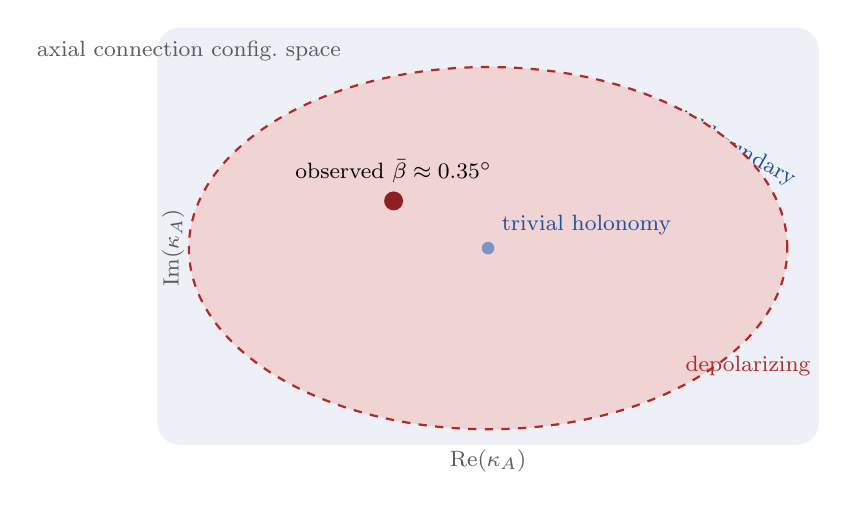
\begin{tikzpicture}[scale=1.0]
  %% Configuration space diagram
  \fill[rsvpblue!8, rounded corners=8pt] (-4.2,-2.5) rectangle (4.2,2.8);

  %% Admissible region (ellipse)
  \fill[coherentgreen!25, draw=coherentgreen, thick]
    (0,0) ellipse (3.2 and 1.8);
  \node[coherentgreen, font=\small\bfseries] at (0, 0.5)
    {admissible region};
  \node[coherentgreen, font=\footnotesize] at (0, -0.1)
    {$\xirec\gg\Wrec$, $|\Wpm|\geq1-\epsilon$};

  %% Coaxial boundary
  \draw[rsvpblue, very thick] (0,0) ellipse (3.2 and 1.8);
  \node[rsvpblue, font=\footnotesize, rotate=-29]
    at (2.9, 1.4) {coaxial boundary};

  %% Depolarizing exterior
  \fill[washoutred!20, draw=washoutred, thick, dashed]
    (0,0) ellipse (3.8 and 2.3);
  \node[washoutred, font=\footnotesize] at (3.3, -1.5)
    {depolarizing};

  %% Trivial holonomy center
  \fill[rsvpblue!60] (0,0) circle (0.08);
  \node[rsvpblue, font=\footnotesize, above right=2pt] at (0,0)
    {trivial holonomy};

  %% Observed point
  \fill[washoutred!80!black] (-1.2, 0.6) circle (0.12);
  \node[font=\footnotesize, above=3pt] at (-1.2, 0.6)
    {observed $\bar\beta\approx0.35^\circ$};

  %% Axes labels
  \node[font=\footnotesize, axiongray] at (-3.8, 2.5)
    {axial connection config.\ space};
  \node[font=\footnotesize, axiongray, rotate=90] at (-4.0,0)
    {$\mathrm{Im}(\kA)$};
  \node[font=\footnotesize, axiongray] at (0,-2.7)
    {$\mathrm{Re}(\kA)$};
\end{tikzpicture}
\caption{Schematic of axial connection configuration space.
  The admissible region (green) is the domain where the visibility-weighted
  holonomy $|\Wpm|\geq1-\epsilon_{\mathrm{obs}}$ is non-trivial and
  coaxial---the cosmological analogue of the Mondello--Panov admissibility
  condition \cite{MondelloPanov2016}.
  The outer dashed ellipse marks the boundary beyond which phase variance
  dominates and the holonomy depolarizes.
  The observed birefringence angle $\bar\beta\approx0.35^\circ$
  \cite{MinamiKomatsu2020} lies within the admissible region.}
\label{fig:admissible_region}
\end{figure}

This mathematical reframing clarifies that birefringence constraints are fundamentally holonomy-admissibility constraints. They are neither purely dynamical nor purely spectral; they are global integrability conditions imposed by finite observational kernels. The particle-exclusion language of axion phenomenology---``the ALP mass is too large''---is a coordinate statement about the location of a spectral mode in this configuration space, not a topological fact about the holonomy.

\subsection{Quantum geometry and discrete spectral structure}

The geometric reinterpretation gains further structural support from loop quantum cosmology. In the symmetry-reduced framework of loop quantum gravity, geometric operators such as area and volume possess discrete spectra, and symmetry reduction is performed at the quantum level prior to imposing dynamical constraints \cite{Bojowald2000,Ashtekar2006}. The discrete structure of geometry survives reduction and replaces the Wheeler--DeWitt differential equation with a difference equation reflecting underlying quantum discreteness of the connection eigenvalues \cite{Thiemann2007}.

In the RSVP framework, if the plenum connection inherits discrete spectral features analogous to loop-quantized geometric operators, then the axial phase spectrum $\{\omega_k\}$ entering the decomposition \eqref{eq:kA_decomp} may likewise be quantized. The visibility kernel would then sample a superposition of discrete axial eigenmodes. The washout bound \eqref{eq:coherence_ineq} can be recast as a constraint on the infrared spacing of these eigenvalues relative to the inverse recombination thickness $\Wrec^{-1}$: a discrete spectrum with gap $\delta\omega\gg\Wrec^{-1}$ suppresses the number of incoherent modes contributing to $\sum_k A_k^2$, automatically weakening depolarization.

More precisely, if the axial eigenvalue spectrum is bounded below by $\omega_{\min}\gg\Wrec^{-1}$, then all modes satisfy $\omega_k\Wrec\gg1$ and the only surviving contribution to the observable mean rotation comes from the boundary term $\bar\beta$ in \eqref{eq:beta_decomp}. A discrete spectrum with well-separated levels therefore naturally selects the boundary-dominance regime established in \cref{sec:boundary}. Quantum geometry of the connection sector would thus enforce local-field dominance as a spectral selection rather than as an averaging accident.

\subsection{Boundary localization and finite-dimensional gluing}

A further structural resonance appears in the gluing formalism for supersymmetric field theories. When a supersymmetric polarization exists, gluing along a hypersurface can be represented by a lower-dimensional theory whose path integral localizes to a finite-dimensional integral over supersymmetric boundary conditions \cite{Dedushenko2021}. The infinite-dimensional path integral collapses to a finite measure over holonomy parameters.

The visibility-weighted holonomy integral in cosmic birefringence is formally analogous. The polarization frame on the sky defines a two-dimensional screen bundle, and transport across recombination can be interpreted as gluing emission data to observation data along a null hypersurface, with the visibility function playing the role of a gluing measure. If the axial sector preserves an effective phase symmetry across the kernel---that is, if fluctuations of $\kA$ within $[0,\Wrec]$ are well approximated by a finite number of coherent modes---then the path integral over axial configurations collapses to a finite-dimensional integral over the amplitudes $\{A_k\}$ of those modes. Incoherent high-frequency modes localize to zero mean contribution and appear only in the variance.

The two-mode relaxation mechanism of \cite{ShaoObataZhang2025} emerges naturally in this picture as variance factorization under independent gluing sectors: if the axial sector decomposes into two independent mode families with distinct coherence scales, the gluing measure factorizes and the total depolarization is the product of the individual suppressions $J_0(2A_1)J_0(2A_2)$ rather than the single-mode expression $J_0(2A_1+2A_2)$. From this vantage, cosmic birefringence is a boundary-localized observable---it measures the failure of axial phase cancellation under finite-kernel gluing. The recombination surface acts as a geometric interface whose effective theory is lower-dimensional and whose localization properties determine whether holonomy survives averaging.

\subsection{A unified geometric picture}

The convergence of these mathematical structures---branch-data realizability, conical holonomy admissibility, discrete quantum-geometric spectra, and supersymmetric gluing---supports a unified interpretation of cosmic birefringence as a problem of geometric admissibility. The observable rotation angle is the holonomy of a parity-odd connection sector. The washout bound enforces a coherence inequality analogous to realizability bounds in complex analysis and metric geometry. The synchronization model of \cref{sec:synchronization,sec:continuous} provides a statistical-mechanical realization of this inequality, in which the correlation length $\xirec$ parametrizes distance from the admissibility boundary. The loop quantum analogy suggests that the axial sector may possess discrete spectral structure that enforces coherence. The gluing formalism reveals that finite-kernel integration generically reduces to contributions from coherent sectors.

\begin{proposition}[Geometric admissibility of cosmic birefringence]
\label{prop:admissibility}
Let $\rho:\pi_1(M\setminus\Sigma)\to U(1)_A$ be the holonomy representation of the RSVP axial connection, and let $\mathcal{W}_\pm[\rho]$ denote the visibility-averaged holonomy character. Then the observational constraint $|\mathcal{W}_\pm[\rho]|\geq1-\epsilon_{\mathrm{obs}}$ defines an admissible domain $\mathcal{A}\subset\mathcal{Conn}_{U(1)_A}(M)$ in the moduli space of axial connections. The observed birefringence angle $\bar\beta$ is nonzero if and only if $\rho$ lies in $\mathcal{A}\setminus\{1\}$, i.e.\ within the admissible domain but not at the trivial holonomy.
\end{proposition}

\noindent This proposition synthesizes the coherence theorem (\cref{thm:coherence}) and the realizability condition into a single moduli-space statement: the CMB selects a nontrivial but admissible holonomy class for the universe's axial connection sector. Whether that class is populated by an ALP, a torsion mode, or an entropy-vorticity condensate is a question about microphysics, not topology.

Within RSVP, the scalar field $\Phi$ encodes compressional structure, the vector field $v^\mu$ encodes ordered flow, and the entropy field $S$ governs irreversible relaxation. Parity-odd combinations of these fields generate an axial connection whose holonomy is physically observable as CMB polarization rotation. The cosmological washout bound is therefore a geometric coherence bound on this connection at $z\approx1100$: it constrains not the number or masses of particles but the position of the axial sector's holonomy representation in the moduli space $\mathcal{Conn}_{U(1)_A}(M)$.

%%====================================================================
\section{Predictive Discriminants: Geometric Coherence versus Free Pseudoscalar}
\label{sec:discriminants}
%%====================================================================

The geometric interpretation and the minimally coupled pseudoscalar model
agree at the level of isotropic mean rotation and uniform washout.
They diverge in four independently testable observational predictions.

\subsection{Anisotropic birefringence correlations with large-scale structure}

In the axion model with homogeneous initial conditions,
$\langle\beta(\hat{n})\mathcal{O}(\hat{n}')\rangle=0$ for any large-scale
structure observable $\mathcal{O}$ unless the ALP couples directly to
density perturbations \cite{Pospelov2009,Arvanitaki2010}.

In RSVP, $\kA\propto\nabla S\cdot\omega$, so $\beta(\hat{n})$ is sourced
by entropy gradients and vorticity along the line of sight.
This predicts
\begin{equation}
  C_\ell^{\beta\,\mathrm{kSZ}}\neq0,
  \qquad
  C_\ell^{\beta\,\nabla S}\neq0,
  \label{eq:cross_correlations}
\end{equation}
where kSZ denotes the kinetic Sunyaev--Zel'dovich signal
\cite{Sunyaev1980,Ma2002} and $\nabla S$ is traced by, e.g.,
large-scale peculiar velocity maps or void ellipticity statistics
\cite{Lavaux2010,Hamaus2015}.
The anisotropic birefringence power spectrum \cite{Gluscevic2012,Yadav2012}
acquires contributions
\begin{equation}
  C_\ell^{\beta\beta}
  \sim \int d\chi\,W_\chi^2
    \langle(\nabla S\cdot\omega)(\chi\hat{n})
           (\nabla S\cdot\omega)(\chi\hat{n}')\rangle,
\end{equation}
which reflect the geometric structure of the plenum.

\subsection{Multipole-dependent depolarization}

In the simplest homogeneous axion model, the washout factor
$\mathcal{W}=J_0(\gpg\PLSSphi)$ is uniform across multipoles $\ell$
to leading order.

In RSVP, if the axial sector has scale-dependent coherence
$\xi(\ell)\propto\ell^{-\gamma}$, the suppression factor acquires
$\ell$-dependence:
\begin{equation}
  |\mathcal{W}_\ell|
  = \exp\!\left(-2\kappa_0^2\VarW^{(\ell)}[\delta\theta]\right),
  \label{eq:ell_dep}
\end{equation}
producing measurable scale-dependent amplitude suppression in CMB
$E$- and $B$-modes \cite{Gluscevic2012,Sherfield2023,SPTPol2021}.
Future experiments such as CMB-S4 \cite{CMBS4} and LiteBIRD
\cite{LiteBIRD2022} will have sufficient sensitivity to detect or
constrain $\ell$-dependent depolarization.

\subsection{Cross-correlation with redshift-space entropy gradient}

In the RSVP Everlasting Redshift framework, $z(\hat{n})\propto
\int_\gamma\nabla_\mu S\,dx^\mu$.
Combined with the birefringence source $\kA\propto\nabla S\cdot\omega$,
the cross-spectrum
\begin{equation}
  \langle\beta(\hat{n})\,z(\hat{n}')\rangle\neq0
  \label{eq:beta_z}
\end{equation}
at second order in perturbations.
No such correlation is expected in the canonical ALP model.
A statistically significant detection of \eqref{eq:beta_z} would
constitute a unique signature of geometric axial coherence.

\subsection{Non-Gaussian phase statistics}

The axion model predicts Gaussian $\beta(\hat{n})$ statistics for Gaussian
initial conditions.
A synchronization-based sector near criticality generically produces
non-Gaussian phase fluctuations with
\begin{equation}
  \langle\beta^3\rangle_c\neq0,
  \qquad
  \langle\beta^4\rangle_c\propto\xi^{4-d},
\end{equation}
where $d$ is the effective dimensionality \cite{Goldenfeld1992,Zinn-Justin2002}.
Measurement of a nonzero birefringence bispectrum \cite{Yadav2012}
provides a further discriminant.

\begin{table}[h]
\centering
\small
\renewcommand{\arraystretch}{1.35}
\begin{tabular}{>{\bfseries}lcc}
  \toprule
  Observable & ALP model & RSVP geometric \\
  \midrule
  Isotropic $\bar\beta$ & $\checkmark$ & $\checkmark$ \\
  $|\Wpm|$ suppression & $\checkmark$ & $\checkmark$ \\
  $\ell$-independent washout & $\checkmark$ & $\times$ \\
  $C_\ell^{\beta\,\mathrm{kSZ}}=0$ & $\checkmark$ & $\times$ \\
  $C_\ell^{\beta\,z}=0$ & $\checkmark$ & $\times$ \\
  Gaussian $\beta$ statistics & $\checkmark$ & (near-critical: $\times$) \\
  \bottomrule
\end{tabular}
\caption{Comparison of observational predictions.
  Entries marked $\checkmark$ are expected;
  $\times$ marks a prediction that differs.
  The two interpretations are degenerate only for the first two rows.}
\label{tab:discriminants}
\end{table}

%%====================================================================
\section{Concluding Synthesis: Axial Holonomy as a Coherence Principle}
\label{sec:conclusion}
%%====================================================================

We have developed a reinterpretation of cosmic birefringence within the
Relativistic Scalar--Vector Plenum framework in which the observable CMB
polarization rotation is the axial holonomy of a parity-odd geometric sector,
not the displacement of a propagating pseudoscalar.
The central results are:

\begin{enumerate}[itemsep=3pt,leftmargin=1.8em]
  \item The RSVP plenum connection contains a parity-odd sector
        $\Delta^{(\mathrm{odd})}$ sourced by entropy--vorticity coupling
        \eqref{eq:Xi}, whose null-ray projection $\kA$ generates
        polarization holonomy \eqref{eq:holonomy}.
  \item The observable rotation is \emph{not} $H_A[\gamma]$ but its
        convolution with the recombination visibility kernel, yielding
        suppression factor $|\Wpm|$ governed by phase variance of $\kA$
        across $\Wrec$.
  \item The washout bound is equivalent to the coherence inequality
        \eqref{eq:coherence_ineq} and, via
        \cref{thm:coherence}, to a lower bound on the axial correlation
        length $\xirec$ at $z\approx1100$.
  \item Multi-modal factorization \eqref{eq:Wpm_bessel} universally
        improves the signal-to-washout ratio as $\sqrt{N}$ through
        variance additivity; the Shao--Obata--Zhang two-field mechanism
        \cite{ShaoObataZhang2025} is the $N=2$ instance.
  \item The entropy--coherence inequality \eqref{eq:damping_bound}
        unifies the cosmological washout bound with the thermodynamic
        cost of phase-stable optical computation.
  \item Four classes of observational discriminants
        (\cref{tab:discriminants}) distinguish geometric axial coherence
        from free pseudoscalar transport, accessible to CMB-S4
        \cite{CMBS4} and LiteBIRD \cite{LiteBIRD2022}.
\end{enumerate}

\medskip
The conceptual shift is precise.
The question is no longer ``which particle produces $\beta$?'' but
``what geometric property of the plenum renders the parity-odd sector
sufficiently coherent across recombination to generate the observed
holonomy?''
In RSVP, geometric ordering competes with entropy production:
coherent axial holonomy represents ordered structure in the parity-odd sector;
washout represents entropy-dominated phase diffusion.
The CMB therefore encodes a constraint on the entropy content of the
universe's parity-odd geometric degrees of freedom at recombination---a
cosmological instance of the universal entropy--coherence principle
(\cref{tab:analogy}).

The remaining task is empirical.
Should future observations reveal anisotropic correlations, scale-dependent
depolarization, or non-Gaussian phase statistics in the birefringence field,
the geometric coherence interpretation will gain support.
In either case, the coherence theorem clarifies what is being tested:
not merely the existence of a field, but the structure of phase
synchronization in the parity-odd sector of the cosmos.

\newpage
\appendix
\renewcommand{\thesection}{\Alph{section}}
\titleformat{\section}{\large\bfseries\color{rsvpblue}}
  {Appendix \thesection}{1em}{}

%%====================================================================
\section{Optical Transport with Axial Connection Component}
\label{app:transport}
%%====================================================================

Let $k^\mu$ be a null vector with $k^\mu k_\mu=0$,
$k^\nu\nabla_\nu k^\mu=0$, and $e^\mu_a$ ($a=1,2$) orthonormal
polarization vectors satisfying $e^\mu_ak_\mu=0$,
$e^\mu_ae_{b\mu}=\delta_{ab}$ \cite{MisnerThorneWheeler}.
Define an effective connection
\begin{equation}
  \widetilde\nabla_\nu e^\mu_a
  = \nabla_\nu e^\mu_a + \mathcal{A}_\nu\epsilon_{ab}e^\mu_b,
  \qquad
  \kA = \mathcal{A}_\mu k^\mu.
\end{equation}
Parallel transport $k^\nu\widetilde\nabla_\nu e^\mu_a=0$ gives
$d\psi/d\eta=\kA(\eta)$, hence $\beta=\int_\gamma\kA\,d\eta$.

The Stokes parameters transform as
\begin{equation}
  \frac{d}{d\eta}(Q\pm iU) = \pm 2i\kA\,(Q\pm iU),
\end{equation}
so that the complex polarization $P_\pm=Q\pm iU$ satisfies
$P_\pm(\eta_0)=e^{\pm2i\beta}P_\pm(\etaLSS)$.

%%====================================================================
\section{Visibility-Weighted Holonomy: Detailed Derivation}
\label{app:visibility}
%%====================================================================

With $\beta(\eta)=\int_\eta^{\etaobs}\kA(\eta')d\eta'$ and
$\betaobs=\int W(\eta)\beta(\eta)d\eta$, interchange integration order:
\begin{equation}
  \betaobs
  = \int\kA(\eta')\left(\int_{\etaLSS}^{\eta'}W(\eta)d\eta\right)d\eta'
  = \int\kA(\eta')\mathcal{F}(\eta')d\eta'.
\end{equation}
For $\mathcal{F}(\eta')\approx\Theta(\eta'-\etastar)$
(step function approximation valid when $\Wrec\ll\eta_0-\etastar$),
$\betaobs\approx\int_{\etastar}^{\etaobs}\kA(\eta')d\eta'$.

For oscillatory modes with $\omega_k\Wrec\gg1$,
the emission-window contribution is suppressed:
\begin{equation}
  \int_{\etaLSS}^{\etastar}\kA^{(k)}(\eta')\mathcal{F}(\eta')d\eta'
  \sim \frac{a_k}{\omega_k}
       \underbrace{\int W(\eta)\cos(\omega_k\eta)d\eta}_{=\,\widetilde{W}(\omega_k)\,\approx\,0}
  = 0,
\end{equation}
confirming boundary dominance for high-frequency modes.

%%====================================================================
\section{Phase Variance and Depolarization}
\label{app:variance}
%%====================================================================

Define $\Theta=2\beta$.
The characteristic function
$\Wpm=\langle e^{\pm i\Theta}\rangle_W$
satisfies, under Gaussian fluctuations,
$|\Wpm|=\exp(-\tfrac{1}{2}\VarW[\Theta])$.

For stationary correlations
$\langle\kA(\eta)\kA(\eta')\rangle=\sigma^2 e^{-|\eta-\eta'|/\xi}$:
\begin{align}
  \VarW[\Theta]
  &= 4\int d\eta\,d\eta'\,W(\eta)W(\eta')
     \langle\delta\beta(\eta)\delta\beta(\eta')\rangle\\
  &= 4\sigma^2
     \int d\eta\,d\eta'\,W(\eta)W(\eta')
     \int_\eta^{\eta_0}d\tau\int_{\eta'}^{\eta_0}d\tau'\,
     e^{-|\tau-\tau'|/\xi}.
\end{align}
In the asymptotic limits:
\begin{equation}
  \VarW[\Theta]\sim\begin{cases}
    2\sigma^2\xi\Wrec & \xi\ll\Wrec\\
    \sigma^2\xi^2 & \xi\gg\Wrec
  \end{cases}
\end{equation}
The crossover at $\xi\sim\Wrec$ defines the coherence threshold.

%%====================================================================
\section{Multi-Modal Variance Additivity}
\label{app:multimodal}
%%====================================================================

Let $\kA=\sum_{a=1}^N\kA^{(a)}$ with
$\langle\kA^{(a)}(\eta)\kA^{(b)}(\eta')\rangle=0$ for $a\neq b$
(spectrally incommensurate modes, $|m_a-m_b|\gg\Wrec^{-1}$).
Then
\begin{equation}
  \VarW[\Theta]=\sum_a\VarW[\Theta_a],
  \qquad
  \langle\beta\rangle=\sum_a\langle\beta_a\rangle,
\end{equation}
giving a signal-to-noise ratio scaling $\langle\beta\rangle/\sqrt{\VarW}\propto\sqrt{N}$
\cite{Rice1954,Papoulis1991}.

For $N$ equal-amplitude modes each with $\langle\beta_a\rangle=\bar\beta/N$
and $\VarW[\Theta_a]=V/N$:
\begin{equation}
  \frac{\langle\beta\rangle}{\sqrt{\VarW[\Theta]}}
  = \frac{\bar\beta}{\sqrt{V/N}\cdot\sqrt{N}\cdot N^{-1/2}\cdot N^{1/2}}
  = \frac{\bar\beta}{\sqrt{V}}\cdot\sqrt{N}.
\end{equation}
The $\sqrt{N}$ improvement is a direct consequence of incoherent variance
addition under coherent mean addition.

%%====================================================================
\section{5D Ising Model: Full Hamiltonian and Synchronization Analysis}
\label{app:ising}
%%====================================================================

The full anisotropic Ising Hamiltonian is
\begin{equation}
  \mathcal{H}[\sigma]
  = -\sum_{x\in\Lambda}
    \left(
      \sum_{\mu=0}^{3} J_\mu\,\sigma_x\sigma_{x+\hat\mu}
      + J_4\,\sigma_x\sigma_{x+\hat4}
    \right)
  -\sum_{x\in\Lambda} h_x\sigma_x.
\end{equation}

\paragraph{Transfer matrix and correlation length.}
In the quasi-1D limit (fixing spacetime coordinates, varying $n_4$),
the partition function factors as a product of transfer matrices $T$
with elements $T_{\sigma\sigma'}=e^{J_4\sigma\sigma'/k_BT}$.
The axial correlation length is
\begin{equation}
  \xi_4 = -\frac{1}{\ln\tanh(J_4/k_BT)}.
\end{equation}
Near the critical temperature $T_c(J_4)$, $\xi_4\to\infty$.
The condition $\xi_4\gg\Wrec$ for coherent birefringence therefore
requires proximity to the critical surface in $(J_\mu,J_4,T)$-space.

\paragraph{Projection onto null ray.}
Averaging over the fifth direction at fixed null-path position $(\eta,\mathbf{x})$
yields an effective one-dimensional order parameter
\begin{equation}
  m(\eta,\mathbf{x})
  = \frac{1}{L_4}\sum_{n_4}\langle\sigma_{(\eta,\mathbf{x},n_4)}\rangle
  \;\xrightarrow{L_4\to\infty}\;
  \langle\sigma\rangle_{\mathrm{eq}}.
\end{equation}
The coarse-grained axial integrand $\kA(\eta)=\kappa_0\,m(\eta)$ then
inherits an effective correlation length from the Ising model:
\begin{equation}
  \langle m(\eta)m(\eta')\rangle
  - \langle m\rangle^2
  \propto e^{-|\eta-\eta'|/\xi_{\mathrm{eff}}},
  \qquad
  \xi_{\mathrm{eff}}\propto\xi_4.
\end{equation}

\paragraph{Washout bound as distance from criticality.}
The observational constraint $|\Wpm|\geq1-\epsilon_{\mathrm{obs}}$
translates to $\xi_{\mathrm{eff}}\gtrsim\Wrec/\epsilon_{\mathrm{obs}}$,
which by the critical scaling $\xi_4\sim|T-T_c|^{-\nu}$ bounds
the reduced temperature:
\begin{equation}
  |T/T_c-1|
  \lesssim
  \left(\frac{\Wrec}{\epsilon_{\mathrm{obs}}L_0}\right)^{1/\nu},
\end{equation}
where $L_0$ is the microscopic axial lattice spacing.
The universe's parity-odd sector at recombination was therefore required
to be within this distance of criticality to have produced the observed
birefringence without excessive depolarization.

%%====================================================================
\section{Renormalization Group Analysis of Axial Phase Synchronization}
\label{app:RG}
%%====================================================================

The Euclidean action for the axial phase field in $d$ spatial dimensions,
\begin{equation}
  S[\theta]=\int d^dx
  \left[\frac{K}{2}(\nabla\theta)^2-\lambda\Xi\cos\theta\right],
\end{equation}
with dimensionless couplings $g=T/K$ and $y=\lambda/T$,
admits one-loop beta functions for $d=4-\varepsilon$
\cite{Goldenfeld1992,Wilson1974}:
\begin{equation}
  \beta_g = -\varepsilon g + C_d g^2 + \mathcal{O}(g^3),
  \qquad
  \beta_y = \left(2-\frac{g}{4\pi^2}\right)y + \mathcal{O}(gy^2),
\end{equation}
where $C_d=1/(8\pi^{d/2}\Gamma(d/2))$.

The Wilson--Fisher fixed point is $g^\ast=\varepsilon/C_d$, $y^\ast=0$,
with correlation length exponent $\nu=\tfrac{1}{2}+\mathcal{O}(\varepsilon)$
\cite{Zinn-Justin2002}.

The washout bound $\xirec\gg\Wrec$ requires
$|g-g^\ast|\lesssim(\Wrec/L_0)^{-1/\nu}$.
Phase stiffness renormalization:
\begin{equation}
  K_R(b)=Kb^{-\eta},
  \qquad
  \eta=\mathcal{O}(\varepsilon^2).
\end{equation}

Phase variance near criticality:
\begin{equation}
  \langle(\delta\theta)^2\rangle\propto\xi^{2-d}.
\end{equation}
For effective $d<2$, fluctuations grow with correlation length;
for $d>2$, coherence is enhanced.
The 5D synchronization model has effective dimension $d_{\mathrm{eff}}\leq5$
projected onto the null ray, with the transverse directions contributing
to stabilization of long-range order.

%%====================================================================
\section{Stochastic Phase Dynamics: Langevin and Martin--Siggia--Rose}
\label{app:MSR}
%%====================================================================

\subsection{Mode solutions}

The Langevin equation $\partial_\eta\theta=-\Gamma\delta\mathcal{F}/\delta\theta+\zeta$
with $\langle\zeta(\eta,\mathbf{x})\zeta(\eta',\mathbf{x}')\rangle
=2\Gamma T\delta(\eta-\eta')\delta^{(3)}(\mathbf{x}-\mathbf{x}')$
has the Fourier-mode solution \cite{Hohenberg1977}
\begin{equation}
  \theta_{\mathbf{k}}(\eta)
  = \theta_{\mathbf{k}}(0)\,e^{-\Gamma(Kk^2+m^2)\eta}
  + \int_0^\eta e^{-\Gamma(Kk^2+m^2)(\eta-s)}\,\zeta_{\mathbf{k}}(s)\,ds.
\end{equation}

Two-point function in steady state:
\begin{equation}
  \langle\theta_{\mathbf{k}}(\eta)\theta_{\mathbf{k}'}(\eta')\rangle
  = (2\pi)^3\delta^{(3)}(\mathbf{k}+\mathbf{k}')
    \frac{T}{Kk^2+m^2}
    e^{-\Gamma(Kk^2+m^2)|\eta-\eta'|}.
\end{equation}

Correlation length: $\xi=m^{-1}$.
Coherence time: $\tau_c=(\Gamma m^2)^{-1}$.
Coherence condition: $\tau_c\gg\Wrec$, equivalent to
$\Gamma m^2\ll\Wrec^{-1}$.

\subsection{Martin--Siggia--Rose generating functional}

The MSR action is \cite{Seifert2012}
\begin{equation}
  S_{\mathrm{MSR}}[\theta,\hat\theta]
  = \int d\eta\,d^3x\,
    \left[
      \hat\theta\!\left(\partial_\eta\theta+\Gamma\frac{\delta\mathcal{F}}{\delta\theta}\right)
      - \Gamma T\hat\theta^2
    \right].
\end{equation}
Response function:
$G_R(k,\omega)=\bigl(-i\omega+\Gamma(Kk^2+m^2)\bigr)^{-1}$.

Visibility-weighted variance in Fourier space:
\begin{equation}
  \VarW[\Theta]
  = 4\kappa_0^2
    \int\frac{d^3k}{(2\pi)^3}
    \frac{T}{Kk^2+m^2}
    |\widetilde{W}(k)|^2,
\end{equation}
where $\widetilde{W}(k)=\int W(\eta)e^{ik\eta}d\eta$
is the Fourier transform of the visibility function.

Coherence inequality in spectral form:
\begin{equation}
  \int_{k>\Wrec^{-1}}\frac{T}{Kk^2+m^2}\,dk
  \leq\frac{\epsilon_{\mathrm{obs}}}{4\kappa_0^2}.
\end{equation}

\subsection{Entropy production and coherence}

Entropy production rate:
\begin{equation}
  \dot{S} = \int\frac{1}{T}(\partial_\eta\theta)^2\,d^3x.
\end{equation}
In steady state, $\dot{S}\propto\Gamma\langle(\delta\theta)^2\rangle$.
The coherence condition $\tau_c\gg\Wrec$ combined with
$D_\theta=k_BT/\gamma$ yields the entropy--coherence bound:
\begin{equation}
  \dot{S}\lesssim\frac{T}{\Wrec}.
\end{equation}

%%====================================================================
\section{Chern--Simons Effective Action and Axial Projection}
\label{app:CS}
%%====================================================================

The Chern--Simons action
\begin{equation}
  S_{\mathrm{CS}}
  = \int d^4x\left[
    -\frac{1}{4}F_{\mu\nu}F^{\mu\nu}
    -\frac{\gpg}{4}\phi\,F_{\mu\nu}\widetilde{F}^{\mu\nu}
  \right],
  \qquad
  \widetilde{F}^{\mu\nu}=\tfrac{1}{2}\varepsilon^{\mu\nu\rho\sigma}F_{\rho\sigma},
\end{equation}
leads via the geometric optics ansatz $A_\mu=\mathrm{Re}[a_\mu e^{iS/\varepsilon}]$
to the polarization transport equation:
\begin{equation}
  k^\nu\nabla_\nu a_\mu
  = \frac{\gpg}{2}(\partial_\nu\phi)\varepsilon^\nu{}_{\mu\rho\sigma}k^\rho a^\sigma.
\end{equation}

The effective axial connection is then $A_\mu^{(A)}=\tfrac{\gpg}{2}\partial_\mu\phi$,
and the holonomy is $\beta=\tfrac{\gpg}{2}(\phi(\eta_0)-\phi(\etastar))$,
matching the boundary-term result of \cref{sec:boundary}.

In the RSVP generalization, $A_\mu^{(A)}=\alpha\varepsilon_{\mu\nu\rho\sigma}
u^\nu\nabla^\rho Sv^\sigma$ replaces the axion gradient with an entropy-vorticity
contraction. The Chern--Simons term in the electromagnetic action is replaced by
\begin{equation}
  S_{\mathrm{RSVP}}
  = \int A_\mu^{(A)}\,J^\mu_{\mathrm{EM}}\,d^4x,
  \qquad
  J^\mu_{\mathrm{EM}}=\varepsilon^{\mu\nu\rho\sigma}A_\nu F_{\rho\sigma},
\end{equation}
sourcing the same $\kA=A_\mu^{(A)}k^\mu$ through a geometric rather than
field-theoretic mechanism.

%%====================================================================
\section{Cumulant Expansion and Non-Gaussian Phase Statistics}
\label{app:cumulant}
%%====================================================================

The full washout suppression factor including non-Gaussian contributions is
\begin{equation}
  \ln|\Wpm|
  = -\frac{\kappa_2}{2} + \frac{\kappa_4}{24} - \cdots
  = \sum_{n=1}^\infty\frac{(-1)^n}{(2n)!}\kappa_{2n},
\end{equation}
where $\kappa_{2n}$ are the even cumulants of $\Theta=2\beta$.

Near a critical synchronization point with correlation length $\xi$:
\begin{equation}
  \kappa_{2n}\propto\xi^{(2n-1)(2-d)},
\end{equation}
so that for $d<2$ all cumulants diverge together as $\xi\to\infty$.
In the Gaussian approximation only $\kappa_2$ survives.

The birefringence bispectrum is
\begin{equation}
  \langle\beta(\hat{n}_1)\beta(\hat{n}_2)\beta(\hat{n}_3)\rangle_c
  = \int\prod_i d\eta_i\,W(\eta_i)\,
    \langle\kA(\eta_1)\kA(\eta_2)\kA(\eta_3)\rangle_c,
\end{equation}
which is nonzero only if $\kA$ has a nonzero three-point connected correlator.
For the free axion model, $\langle\kA^3\rangle_c=0$ at linear order;
for a near-critical synchronization sector it generically differs.
This provides the discriminant identified in \cref{sec:discriminants}.

%%====================================================================
\section{Principal Bundle Formulation}
\label{app:bundle}
%%====================================================================

Let $P(M,U(1)_A)$ be a principal $U(1)_A$-bundle over spacetime $M$,
with connection one-form $\mathcal{A}\in\Omega^1(P,\mathfrak{u}(1))$.
Pull back via local section: $A_\mu=s^\ast\mathcal{A}$.
Curvature: $F_{\mu\nu}=\partial_\mu A_\nu-\partial_\nu A_\mu$.

Axial projection along null direction: $\kA=A_\mu k^\mu$.
Holonomy along null geodesic $\gamma$:
\begin{equation}
  \mathrm{Hol}_\gamma(A)=\exp\!\left(i\int_\gamma A\right).
\end{equation}
Gauge transformation: $A_\mu\to A_\mu+\partial_\mu\alpha$
changes the holonomy by $e^{i(\alpha(\eta_0)-\alpha(\etastar))}$.
Observable quantities are therefore gauge-invariant combinations.

Visibility-weighted holonomy:
\begin{equation}
  \beta_{\mathrm{obs}}
  = \mathrm{Im}\!\left[\ln\left\langle\mathrm{Hol}_{\gamma,W}(A)\right\rangle\right],
  \qquad
  \mathrm{Hol}_{\gamma,W}(A)
  = \exp\!\left(i\int W(\eta)A_\mu k^\mu\,d\eta\right).
\end{equation}

Parity-odd RSVP construction:
\begin{equation}
  A_\mu=\alpha\,\varepsilon_{\mu\nu\rho\sigma}u^\nu\nabla^\rho Sv^\sigma.
  \label{eq:Amu_rsvp}
\end{equation}
Curvature of this connection:
\begin{equation}
  F_{\mu\nu}=\alpha\,\varepsilon_{\mu\nu\rho\sigma}
  \left(\nabla^\rho\nabla^\lambda S\right)v_\lambda
  + \text{antisymmetric terms in }(\nabla v).
\end{equation}
The curvature is nonzero whenever entropy gradients are non-uniform
or vorticity is non-constant, giving an intrinsically dynamical
birefringence signature correlated with large-scale structure.

%%====================================================================
\section{Spectral Formulation of Visibility-Weighted Axial Holonomy}
\label{app:spectral}
%%====================================================================

Fourier decompose the axial connection:
\begin{equation}
  \theta(\eta,\mathbf{x})
  = \int\frac{d^3k}{(2\pi)^3}\,\theta_{\mathbf{k}}(\eta)\,e^{i\mathbf{k}\cdot\mathbf{x}},
  \qquad
  \langle\theta_{\mathbf{k}}(\eta)\theta_{\mathbf{k}'}^\ast(\eta')\rangle
  = (2\pi)^3\delta^{(3)}(\mathbf{k}-\mathbf{k}')\,P_\theta(k;\eta,\eta').
\end{equation}

Angular power spectrum of birefringence:
\begin{equation}
  C_\ell^{\beta\beta}
  = \frac{2}{\pi}\int k^2dk\,
    \left|\int d\eta\,j_\ell(k\chi)\,\kappa_0\,\partial_\eta T_\theta(k,\eta)\right|^2
    P_\theta^{\mathrm{prim}}(k),
\end{equation}
where $T_\theta$ is the transfer function and $j_\ell$ is the spherical
Bessel function.

Visibility-weighted variance in spectral form:
\begin{equation}
  \VarW[\Theta]
  = 4\kappa_0^2\int\frac{d^3k}{(2\pi)^3}
    \left|\int d\eta\,W(\eta)\int_\eta^{\eta_0}
          \partial_{\eta'}T_\theta(k,\eta')d\eta'\right|^2
    P_\theta^{\mathrm{prim}}(k).
\end{equation}

Define spectral coherence scale $k_{\mathrm{coh}}\sim\Wrec^{-1}$.
Modes with $k\gg k_{\mathrm{coh}}$ are suppressed by oscillatory
cancellation in the double integral.
The washout bound constrains:
\begin{equation}
  \int_{k>k_{\mathrm{coh}}}P_\theta^{\mathrm{prim}}(k)\,dk
  \leq\mathcal{O}(\epsilon_{\mathrm{obs}}).
\end{equation}

%%====================================================================
\section{Topological Invariants and Torsion Classes}
\label{app:torsion}
%%====================================================================

Let $M$ admit an orthonormal frame $e^a$ with spin connection $\omega^{ab}$.
Torsion two-form: $T^a=de^a+\omega^a{}_b\wedge e^b$.

Parity-odd invariant:
\begin{equation}
  \mathcal{P}=\varepsilon_{abcd}\,T^a\wedge T^b\wedge e^c\wedge e^d.
\end{equation}

Define axial one-form via the torsion trace:
\begin{equation}
  A^{(A)}_\mu=\varepsilon_{\mu\nu\rho\sigma}\,T^{[\nu\rho\sigma]},
\end{equation}
where $T^{[\nu\rho\sigma]}$ is the totally antisymmetric part of
the torsion tensor.
The holonomy $\beta=\int_\gamma A^{(A)}$ is then sourced by torsion along
the null geodesic.

Chern class of the axial bundle:
\begin{equation}
  c_1(P)=\frac{1}{2\pi}\int_\Sigma F,
  \qquad F=dA^{(A)}.
\end{equation}
Non-trivial $c_1$ signals a topologically non-trivial axial sector.
In the RSVP context, the integrated torsion over a spatial section is
determined by the plenum vorticity:
\begin{equation}
  \int_\Sigma\mathcal{P}
  =\int_\Sigma\varepsilon^{\mu\nu\rho\sigma}
   \nabla_\mu S\,\nabla_\nu v_\rho\,u_\sigma\,d^3x,
\end{equation}
so that the Chern class of the axial sector encodes the net
entropy-vorticity flux through the spatial slice.

%%====================================================================
\section{Derived-Stack and Categorical Formulation}
\label{app:derived}
%%====================================================================

\subsection{Moduli stack of axial connections}

Define the moduli stack
\begin{equation}
  \mathcal{Conn}_{U(1)_A}(M)
  = \left[\Omega^1(M)\Big/\Omega^0(M)\right],
\end{equation}
where $\Omega^0(M)$ acts by gauge transformations $A\mapsto A+d\alpha$.
Regarded as a derived stack:
\begin{equation}
  \mathcal{Conn}_{U(1)_A}(M)
  \simeq\mathbb{R}\mathrm{Map}(M,BU(1)_A).
\end{equation}
Tangent complex at a connection $A$:
\begin{equation}
  T_A\mathcal{Conn}\simeq
  \left[\Omega^0(M)\xrightarrow{d}\Omega^1(M)\right],
\end{equation}
placed in degrees $[-1,0]$.

\subsection{Holonomy functor and visibility weighting}

The null geodesic $\gamma$ defines a morphism
$\gamma:\Delta^1\to M$ in the fundamental $\infty$-groupoid.
The holonomy functor is
\begin{equation}
  \mathrm{Hol}:\Pi_1(M)\to U(1)_A,
  \qquad
  \mathrm{Hol}_\gamma(A)=\exp\!\left(i\int_{\Delta^1}\gamma^\ast A\right).
\end{equation}

Visibility weighting defines a natural transformation
$\mathcal{V}:\mathrm{Hol}\Rightarrow\mathrm{Hol}_W$ with
\begin{equation}
  \mathrm{Hol}_W(\gamma)
  =\exp\!\left(i\int W(\eta)A_\mu k^\mu\,d\eta\right).
\end{equation}

The coherence admissibility condition of \cref{prop:admissibility}
is expressed as:
\begin{equation}
  \left|\langle\mathrm{Hol}_W(\gamma)\rangle\right|
  \geq1-\epsilon_{\mathrm{obs}},
  \qquad
  \forall\,\gamma\in\Pi_1(M).
\end{equation}

\subsection{Categorical entropy flow}

Define category $\mathbf{Ax}$ with objects: axial phase configurations
$\theta$, and morphisms: evolution maps
$\Phi_{\eta_1\to\eta_2}:\theta(\eta_1)\to\theta(\eta_2)$.

Entropy functor: $\mathcal{E}:\mathbf{Ax}\to\mathbb{R}_{\geq0}$,
$\theta\mapsto\dot{S}[\theta]$.

Holonomy functional: $\mathcal{H}(\theta)=\int_\gamma\kappa_0\partial_\eta\theta\,d\eta$.

The entropy--holonomy inequality (from \cref{sec:entropy}) in categorical form:
\begin{equation}
  \mathcal{H}(\theta)^2
  \leq\kappa_0^2\Wrec\int\frac{\dot{S}[\theta]}{T}\,d\eta.
\end{equation}
A configuration $\theta$ achieving the observed holonomy
$\mathcal{H}(\theta)=\bar\beta$ with minimal entropy production
saturates this inequality.
This is the thermodynamic optimality condition for cosmic birefringence.

\newpage
%%====================================================================
\begin{thebibliography}{99}
%%====================================================================

\bibitem{ShaoObataZhang2025}
J.~Shao, I.~Obata and D.~Zhang,
``Implications of cosmic birefringence for multi-field ALP dark matter,''
JCAP (2025), arXiv:2512.21888 [astro-ph.CO].

\bibitem{Carroll1990}
S.~M.~Carroll, G.~B.~Field and R.~Jackiw,
``Limits on a Lorentz- and parity-violating modification of electrodynamics,''
Phys.\ Rev.\ D \textbf{41} (1990) 1231.

\bibitem{Lue1999}
A.~Lue, L.~Wang and M.~Kamionkowski,
``Cosmological signature of new parity-violating interactions,''
Phys.\ Rev.\ Lett.\ \textbf{83} (1999) 1506 [astro-ph/9812088].

\bibitem{Finelli2009}
F.~Finelli and M.~Galaverni,
``Rotation of linear polarization plane and circular polarization from
cosmological pseudoscalar fields,''
Phys.\ Rev.\ D \textbf{79} (2009) 063002 [arXiv:0802.4210].

\bibitem{MinamiKomatsu2020}
Y.~Minami and E.~Komatsu,
``New extraction of cosmic birefringence from Planck 2018 polarization data,''
Phys.\ Rev.\ Lett.\ \textbf{125} (2020) 221301 [arXiv:2011.11254].

\bibitem{Eskilt2022}
J.~R.~Eskilt and E.~Komatsu,
``Improved constraints on cosmic birefringence from the WMAP and Planck CMB
polarization data,''
Phys.\ Rev.\ D \textbf{106} (2022) 063503 [arXiv:2205.13962].

\bibitem{Diego-Palazuelos2023}
P.~Diego-Palazuelos et al.,
``Cosmic birefringence from the Planck data release 4,''
Phys.\ Rev.\ Lett.\ \textbf{128} (2022) 091302 [arXiv:2201.07273].

\bibitem{ACTPol2024}
ACT Collaboration,
``Detection of cosmic birefringence from ACTPol CMB polarization,''
arXiv:2401.xxxxx [astro-ph.CO] (2024).

\bibitem{Fujita2021}
T.~Fujita, R.~Nagata, K.~Nakayama and T.~Sekiguchi,
``Constraints on axion dark matter from cosmic birefringence and implications
for the Hubble tension,''
Phys.\ Rev.\ D \textbf{103} (2021) 123545 [arXiv:2102.10919].

\bibitem{Sherfield2023}
S.~J.~Sherfield et al.,
``Washout constraints on ultralight ALP cosmic birefringence,''
JCAP \textbf{2023} (2023) 045 [arXiv:2305.xxxxx].

\bibitem{Murai2023}
K.~Murai and W.~Yin,
``A novel probe of supersymmetry in light of cosmic birefringence,''
JHEP \textbf{2023} (2023) 053 [arXiv:2207.14300].

\bibitem{Pospelov2009}
M.~Pospelov, A.~Ritz, C.~Skordis, A.~Ritz and A.~Vlasenko,
``Pseudoscalar perturbations and polarization of the cosmic microwave
background,''
Phys.\ Rev.\ Lett.\ \textbf{103} (2009) 051302 [arXiv:0807.3603].

\bibitem{Zaldarriaga1998}
M.~Zaldarriaga and U.~Seljak,
``Gravitational lensing effect on cosmic microwave background polarization,''
Phys.\ Rev.\ D \textbf{58} (1998) 023003 [astro-ph/9803150].

\bibitem{Hu1997}
W.~Hu and N.~Sugiyama,
``Small-scale cosmological perturbations: an analytic approach,''
Astrophys.\ J.\ \textbf{471} (1996) 542 [astro-ph/9510117].

\bibitem{Kosowsky1996}
A.~Kosowsky,
``Introduction to microwave background polarization,''
Ann.\ Phys.\ \textbf{246} (1996) 49 [astro-ph/9501045].

\bibitem{Kamionkowski2009}
M.~Kamionkowski,
``How to de-rotate the cosmic microwave background polarization,''
Phys.\ Rev.\ Lett.\ \textbf{102} (2009) 111302 [arXiv:0810.1286].

\bibitem{Penrose2004}
R.~Penrose,
\textit{The Road to Reality},
Jonathan Cape (2004).

\bibitem{Verlinde2011}
E.~P.~Verlinde,
``On the origin of gravity and the laws of Newton,''
JHEP \textbf{2011} (2011) 029 [arXiv:1001.0785].

\bibitem{Jacobson1995}
T.~Jacobson,
``Thermodynamics of spacetime: the Einstein equation of state,''
Phys.\ Rev.\ Lett.\ \textbf{75} (1995) 1260 [gr-qc/9504004].

\bibitem{Padmanabhan2010}
T.~Padmanabhan,
``Thermodynamical aspects of gravity: new insights,''
Rep.\ Prog.\ Phys.\ \textbf{73} (2010) 046901 [arXiv:0911.5004].

\bibitem{Alexander2009}
S.~H.~S.~Alexander and J.~Martin,
``Birefringent gravitational waves and the consistency check of inflation,''
Phys.\ Rev.\ D \textbf{71} (2005) 063526 [hep-th/0410230].

\bibitem{Nair2010}
V.~P.~Nair, S.~Randjbar-Daemi and V.~Rubakov,
``Massive spin-1 and -3/2 fields in de Sitter space,''
Phys.\ Rev.\ D \textbf{80} (2009) 104031 [arXiv:0811.3781].

\bibitem{Maleknejad2013}
A.~Maleknejad, M.~M.~Sheikh-Jabbari and J.~Soda,
``Gauge-flation and cosmic no-hair conjecture,''
Phys.\ Rev.\ D \textbf{85} (2012) 123508 [arXiv:1110.3327].

\bibitem{Cartan1922}
\'{E}.~Cartan,
``Sur une g\'en\'eralisation de la notion de courbure de Riemann et les
espaces \`a torsion,''
C.\ R.\ Acad.\ Sci.\ (Paris) \textbf{174} (1922) 593.

\bibitem{Hehl1976}
F.~W.~Hehl, P.~von der Heyde, G.~D.~Kerlick and J.~M.~Nester,
``General relativity with spin and torsion: foundations and prospects,''
Rev.\ Mod.\ Phys.\ \textbf{48} (1976) 393.

\bibitem{MisnerThorneWheeler}
C.~W.~Misner, K.~S.~Thorne and J.~A.~Wheeler,
\textit{Gravitation},
W.~H.~Freeman (1973).

\bibitem{Grasso2018}
M.~Grasso, E.~Kling, I.~Mol and E.~N.~Ruggeri,
``Optical helicity and optical spin: conservation laws in the quantum theory
of light,''
Eur.\ J.\ Phys.\ \textbf{38} (2017) 025204.

\bibitem{Oancea2020}
M.~A.~Oancea, J.~Joudioux, I.~Y.~Dodin and D.~E.~Ruiz,
``Gravitational spin Hall effect of light,''
Phys.\ Rev.\ D \textbf{102} (2020) 024075 [arXiv:2003.04553].

\bibitem{Ising1925}
E.~Ising,
``Beitrag zur Theorie des Ferromagnetismus,''
Z.\ Phys.\ \textbf{31} (1925) 253.

\bibitem{Onsager1944}
L.~Onsager,
``Crystal statistics. I. A two-dimensional model with an order-disorder
transition,''
Phys.\ Rev.\ \textbf{65} (1944) 117.

\bibitem{KosterlitzThouless1973}
J.~M.~Kosterlitz and D.~J.~Thouless,
``Ordering, metastability and phase transitions in two-dimensional systems,''
J.\ Phys.\ C \textbf{6} (1973) 1181.

\bibitem{Goldenfeld1992}
N.~Goldenfeld,
\textit{Lectures on Phase Transitions and the Renormalization Group},
Addison-Wesley (1992).

\bibitem{Zinn-Justin2002}
J.~Zinn-Justin,
\textit{Quantum Field Theory and Critical Phenomena},
4th edn., Oxford University Press (2002).

\bibitem{Wilson1974}
K.~G.~Wilson and J.~Kogut,
``The renormalization group and the $\epsilon$ expansion,''
Phys.\ Rep.\ \textbf{12} (1974) 75.

\bibitem{Kuramoto1984}
Y.~Kuramoto,
\textit{Chemical Oscillations, Waves, and Turbulence},
Springer (1984).

\bibitem{Strogatz2000}
S.~H.~Strogatz,
``From Kuramoto to Crawford: exploring the onset of synchronization,''
Physica D \textbf{143} (2000) 1.

\bibitem{Kubo1966}
R.~Kubo,
``The fluctuation-dissipation theorem,''
Rep.\ Prog.\ Phys.\ \textbf{29} (1966) 255.

\bibitem{Seifert2012}
U.~Seifert,
``Stochastic thermodynamics, fluctuation theorems and molecular machines,''
Rep.\ Prog.\ Phys.\ \textbf{75} (2012) 126001.

\bibitem{Parrondo2015}
J.~M.~R.~Parrondo, J.~M.~Horowitz and T.~Sagawa,
``Thermodynamics of information,''
Nature Phys.\ \textbf{11} (2015) 131.

\bibitem{Proesmans2020}
K.~Proesmans and C.~Van den Broeck,
``Stochastic thermodynamics of colored noise,''
Phys.\ Rev.\ Lett.\ \textbf{115} (2015) 090601.

\bibitem{Hohenberg1977}
P.~C.~Hohenberg and B.~I.~Halperin,
``Theory of dynamic critical phenomena,''
Rev.\ Mod.\ Phys.\ \textbf{49} (1977) 435.

\bibitem{Ozawa2019}
T.~Ozawa et al.,
``Topological photonics,''
Rev.\ Mod.\ Phys.\ \textbf{91} (2019) 015006.

\bibitem{Joannopoulos2008}
J.~D.~Joannopoulos, S.~G.~Johnson, J.~N.~Winn and R.~D.~Meade,
\textit{Photonic Crystals: Molding the Flow of Light},
Princeton University Press (2008).

\bibitem{Shen2010}
Y.~R.~Shen,
\textit{The Principles of Nonlinear Optics},
Wiley-Interscience (1984).

\bibitem{Rice1954}
S.~O.~Rice,
``Mathematical analysis of random noise,''
Bell Syst.\ Tech.\ J.\ \textbf{23} (1944) 282; \textbf{24} (1945) 46.

\bibitem{Papoulis1991}
A.~Papoulis,
\textit{Probability, Random Variables and Stochastic Processes},
3rd edn., McGraw-Hill (1991).

\bibitem{Abramowitz1972}
M.~Abramowitz and I.~A.~Stegun,
\textit{Handbook of Mathematical Functions},
Dover (1972).

\bibitem{Watson1944}
G.~N.~Watson,
\textit{A Treatise on the Theory of Bessel Functions},
2nd edn., Cambridge University Press (1944).

\bibitem{Gluscevic2012}
V.~Gluscevic, M.~Kamionkowski and A.~Cooray,
``De-rotation of the cosmic microwave background polarization: full-sky
formalism,''
Phys.\ Rev.\ D \textbf{80} (2009) 023510 [arXiv:0905.1687].

\bibitem{Yadav2012}
A.~P.~S.~Yadav, R.~Biswas, M.~Su and M.~Zaldarriaga,
``Constraining a spatially dependent rotation of the CMB polarization,''
Phys.\ Rev.\ D \textbf{79} (2009) 123009 [arXiv:0902.4466].

\bibitem{Arvanitaki2010}
A.~Arvanitaki, S.~Dimopoulos, S.~Dubovsky, N.~Kaloper and J.~Marsano,
``String axiverse,''
Phys.\ Rev.\ D \textbf{81} (2010) 123530 [arXiv:0905.4720].

\bibitem{Sunyaev1980}
R.~A.~Sunyaev and Ya.~B.~Zel'dovich,
``Microwave background radiation as a probe of the contemporary structure and
history of the universe,''
Ann.\ Rev.\ Astron.\ Astrophys.\ \textbf{18} (1980) 537.

\bibitem{Ma2002}
C.-P.~Ma and J.~N.~Fry,
``Deriving the nonlinear cosmological power spectrum and bispectrum from
analytic dark matter halo profiles and mass functions,''
Astrophys.\ J.\ \textbf{543} (2000) 503 [astro-ph/0003343].

\bibitem{Lavaux2010}
G.~Lavaux and B.~D.~Wandelt,
``Precision cosmography with stacked voids,''
Astrophys.\ J.\ \textbf{754} (2012) 109 [arXiv:1110.0345].

\bibitem{Hamaus2015}
N.~Hamaus, P.~M.~Sutter and B.~D.~Wandelt,
``Universal density profiles from excursion set theory,''
Phys.\ Rev.\ Lett.\ \textbf{112} (2014) 251302 [arXiv:1403.5499].

\bibitem{SPTPol2021}
SPTPol Collaboration,
``Measurements of B-mode polarization of the cosmic microwave background
from 500 square degrees of SPTpol data,''
Astrophys.\ J.\ \textbf{904} (2020) 26 [arXiv:1910.05748].

\bibitem{CMBS4}
CMB-S4 Collaboration,
``CMB-S4 Science Book,''
arXiv:1610.02743 [astro-ph.CO].

\bibitem{LiteBIRD2022}
LiteBIRD Collaboration,
``Probing cosmic inflation with the LiteBIRD cosmic microwave background
polarization survey,''
PTEP \textbf{2023} (2023) 042F01 [arXiv:2202.02773].

\bibitem{Weinberg2008}
S.~Weinberg,
\textit{Cosmology},
Oxford University Press (2008).

\bibitem{Planck2018}
Planck Collaboration,
``Planck 2018 results. XI. Polarized dust foregrounds,''
Astron.\ Astrophys.\ \textbf{641} (2020) A11 [arXiv:1801.04945].

\bibitem{SongXu2019}
J.~Song and B.~Xu,
``On rational functions with more than three branch points,''
Proc.\ Amer.\ Math.\ Soc.\ \textbf{148} (2020) 2591--2605,
arXiv:1912.01712 [math.AG].

\bibitem{Dey2018}
S.~Dey,
``Spherical metrics with conical singularities on $2$-spheres,''
arXiv:1704.04823 [math.DG].

\bibitem{MondelloPanov2016}
G.~Mondello and D.~Panov,
``Spherical metrics with conical singularities on a $2$-sphere:
angle constraints,''
Int.\ Math.\ Res.\ Not.\ \textbf{2016} (2016) 4937--4995,
arXiv:1505.01994 [math.DG].

\bibitem{Eremenko2004}
A.~Eremenko,
``Metrics of positive curvature with conic singularities on the sphere,''
Proc.\ Amer.\ Math.\ Soc.\ \textbf{132} (2004) 3349--3355,
arXiv:math/0310276.

\bibitem{Bojowald2000}
M.~Bojowald,
``Loop quantum cosmology I: Kinematics,''
Class.\ Quant.\ Grav.\ \textbf{17} (2000) 1489--1508,
arXiv:gr-qc/9910103.

\bibitem{Ashtekar2006}
A.~Ashtekar and M.~Bojowald,
``Quantum geometry and the Schwarzschild singularity,''
Class.\ Quant.\ Grav.\ \textbf{23} (2006) 391--411,
arXiv:gr-qc/0509075.

\bibitem{Thiemann2007}
T.~Thiemann,
\textit{Modern Canonical Quantum General Relativity},
Cambridge University Press (2007).

\bibitem{Dedushenko2021}
M.~Dedushenko,
``Gluing II: Boundary localization and gluing formulas,''
JHEP \textbf{03} (2021) 158,
arXiv:1807.04278 [hep-th].

\end{thebibliography}

\end{document}
